% ======================================================================
% Paper D of the meander series: the KPZ formula in a continuum model, and near-splits in the
% conjectured meander limit. Compile with: tectonic main.tex
% Sources: see the appendix "Where the proofs are" (sec_appendix.tex).
% Lines marked "% UNVERIFIED" state less than the sources or flag a point not settled by them.
% ======================================================================
\documentclass[11pt]{article}
% Shared preamble for the meander paper series (papers A-D). Compile each paper with tectonic.
\usepackage[T1]{fontenc}
\usepackage[margin=1.15in]{geometry}
\usepackage{amsmath,amssymb,amsthm}
\usepackage{booktabs,array}
\usepackage{float}
\usepackage{tikz}
\usetikzlibrary{arrows.meta,decorations.pathmorphing,positioning}
\usepackage{pgfplots}
\pgfplotsset{compat=1.16}
\usepackage[colorlinks=true,linkcolor=blue!50!black,citecolor=blue!50!black,urlcolor=blue!50!black]{hyperref}

\newtheorem{theorem}{Theorem}
\newtheorem{proposition}[theorem]{Proposition}
\newtheorem{lemma}[theorem]{Lemma}
\newtheorem{corollary}[theorem]{Corollary}
\newtheorem{conjecture}[theorem]{Conjecture}
\theoremstyle{definition}
\newtheorem{definition}[theorem]{Definition}
\theoremstyle{remark}
\newtheorem*{remark}{Remark}

\emergencystretch=2em
\raggedbottom

% Tapes of the tape machine. Write -{}- for a double minus inside \tape{...} to avoid the
% typewriter dash ligature.
\newcommand{\tape}[1]{\texttt{#1}}
\newcommand{\hd}[1]{\texttt{[#1]}}

% Series line under the title.
\newcommand{\seriesline}[1]{\par\smallskip{\small\itshape Meander numbers: growth rate and exponent. #1}}

% The running example (order 3): upper arches (1,2), (3,6), (4,5); lower arches (1,6), (2,5), (3,4).
\newcommand{\meanderroad}{%
  \draw (1,0) arc[start angle=180,end angle=0,radius=0.5];
  \draw (3,0) arc[start angle=180,end angle=0,radius=1.5];
  \draw (4,0) arc[start angle=180,end angle=0,radius=0.5];
  \draw (1,0) arc[start angle=180,end angle=360,radius=2.5];
  \draw (2,0) arc[start angle=180,end angle=360,radius=1.5];
  \draw (3,0) arc[start angle=180,end angle=360,radius=0.5];
}
\newcommand{\meanderfigure}{%
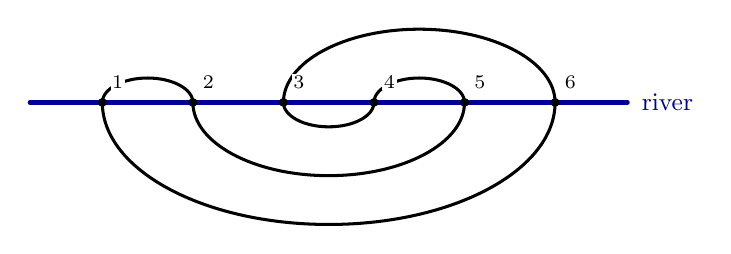
\begin{tikzpicture}[x=1.15cm,y=0.62cm,line cap=round]
  \draw[blue!60!black,line width=1.6pt] (0.2,0)--(6.8,0);
  \node[blue!60!black,anchor=west] at (6.85,0) {\small river};
  \begin{scope}[line width=1.1pt]\meanderroad\end{scope}
  \foreach \k in {1,...,6} {\fill (\k,0) circle[radius=1.6pt]; \node[fill=white,inner sep=0.6pt,font=\scriptsize] at (\k+0.17,0.42) {\k};}
\end{tikzpicture}}

% The series. Each paper cites the others as \cite{PaperA} etc.

\usepackage{enumitem}
\setlist{itemsep=1pt,topsep=4pt,parsep=0pt}

% Local notation.
\newcommand{\Prob}{\mathbb{P}}
\newcommand{\E}{\mathbb{E}}
\newcommand{\Pt}{\mathcal{P}}
\newcommand{\astar}{\alpha_*}
\newcommand{\xstar}{x_*}
\newcommand{\ldet}{\det{}'\Delta_g}
% File names in the appendix table, breakable at slashes and underscores.
\def\UrlBreaks{\do\/\do\_}
\newcommand{\fn}[1]{\nolinkurl{#1}}

\title{The KPZ formula in a continuum model,\\ and near-splits in the conjectured meander limit%
\seriesline{Paper D.}}
\author{Carl Johan Ragnarsson}
\date{Draft of October 25, 2026}

\begin{document}
\maketitle

\begin{abstract}
The number of meanders with $2n$ crossings is conjectured to grow like $A\mu^n n^{-\alpha}$ with
$\alpha=(29+\sqrt{145})/12\approx3.4201$. The value comes from the Knizhnik--Polyakov--Zamolodchikov
(KPZ) formula of physics, applied to a random surface carrying two curves. This paper studies two
continuum settings in which parts of that prediction can be proved. In the random surface model
of Ang, Park, Pfeffer and Sheffield, built by subdividing a square according to a Gaussian free
field, we prove that the probability of at least $n$ squares is $n^{-4/\gamma^2+o(1)}$ for every
value of the parameter, including the critical endpoint. They showed that weighting by a power of
a Laplacian determinant, the continuum analog of counting spanning trees, exactly changes the
parameter. Combined with this and with a normalization identity that we derive, the tail law gives
the full KPZ curve in that model, for the total weight of sizes at least $n$; the analog of two
spanning trees has tail exponent $(17+\sqrt{145})/12$, which corresponds to the predicted
$\alpha_*=(29+\sqrt{145})/12$. We also show that large area does not force many squares, and we discuss a
branching random walk in which the formula is the relation between two exponential rates. In the
random surface with two independent space-filling curves that Borga, Gwynne and Sun conjecture to
be the limit of large meanders, we prove that the probability of a near-split into two halves,
imperfect by a fraction $\delta$, lies between constant multiples of $\delta^{3.4201}$ and
$\delta^{3.1344}$; the exponent of the lower bound is the predicted one. A calculation with two
random disks glued along their boundaries, a simpler surface whose link to near-splits is open,
gives the predicted exponent exactly. None of these results is yet a theorem about finite
meanders; we state what is missing to transfer them, and what the missing steps would give. All code was written using Claude (Opus
5.5) or Codex (Sol 5.1) with active review and guidance throughout.
\end{abstract}


%%%%%%%%%%%%%%%%%%%%%%%%%%%%%%%%%%%%%%%%%%%%%%%%%%%%%%%%%%%%%%%%%%%%%%%%
\section{Introduction}\label{sec:intro}
%%%%%%%%%%%%%%%%%%%%%%%%%%%%%%%%%%%%%%%%%%%%%%%%%%%%%%%%%%%%%%%%%%%%%%%%

\subsection{Meanders and the KPZ formula}

A \emph{meander of order $n$} is a closed curve in the plane, the \emph{road}, that crosses a
fixed straight line, the \emph{river}, exactly $2n$ times and never crosses itself, counted up to
deformations that keep the pattern of crossings. The river cuts the road into \emph{arches}, the
pieces of road between consecutive crossings; the arches above the river pair up the crossings
without crossing each other, and so do the arches below. Let $M_n$ be the number of meanders of
order $n$; the first values are $1,2,8,42$. Two meanders of orders $a$ and $b$ can be \emph{glued
end to end}: place them side by side on one river, remove the upper arch at the last crossing of
the left one and the upper arch at the first crossing of the right one, and reconnect the four
loose ends by a short arch joining these two crossings and a long arch over it. The two roads merge
into one, giving a meander of order $a+b$. Gluing is injective, since the two pieces are recovered
by undoing the reconnection, so $M_{a+b}\ge M_aM_b$, and $\mu=\lim_n M_n^{1/n}=\sup_nM_n^{1/n}$ exists by Fekete's lemma;
numerically $\mu\approx12.26$~\cite{JG}. The leftover factor $u_n=M_n/\mu^n$ is believed
to decay like a power of $n$:
\begin{equation}\label{eq:conj}
M_n\;\approx\;A\,\mu^n n^{-\alpha},\qquad \alpha=\astar=\frac{29+\sqrt{145}}{12}\approx3.4201 .
\end{equation}
This value was predicted by Di~Francesco, Golinelli and Guitter~\cite{DGG}, and numerical
estimates agree with it~\cite{JG}. It has not been proved.

The prediction comes from physics. A large meander is viewed as a random surface carrying two
curves, river and road, that each visit every part of it. The discrete random surfaces here are
\emph{planar maps}: connected graphs drawn on the sphere without edge crossings, counted up to
deformation. Each kind of decoration drawn on a random surface (a spanning tree, a curve, a spin
configuration) has a \emph{central charge} $c$, a number that measures how strongly the decorated
surface prefers round shapes to shapes with thin necks: $c=0$ for a bare surface, $c=-2$ for a
spanning tree and, it is predicted, for a curve through every point. Independent decorations are
expected to add their central charges, so a meander is predicted to have $c=-4$. The
\emph{KPZ formula} of Knizhnik, Polyakov and Zamolodchikov~\cite{KPZ} turns $c$ into an exponent:
\begin{equation}\label{eq:kpz}
\alpha=1+x,\qquad x+\frac1x=\frac{13-c}{6},\qquad x\ge1 .
\end{equation}
Here $x$ is the exponent of a tail: if, after the exponential growth is divided out, surfaces of
size exactly $n$ carry total weight about $n^{-1-x}$, then surfaces of size at least $n$ carry total
weight about $n^{-x}$. At $c=0$ the
formula gives $\alpha=5/2$, the exponent of planar maps found by Tutte~\cite{Tutte}; at $c=-2$ it
gives $\alpha=3$, the exponent of maps with a spanning tree found by Mullin~\cite{Mullin}; at $c=-4$
the equation $x+1/x=17/6$ has the root
\[
\xstar=\frac{17+\sqrt{145}}{12}\approx2.4201,\qquad 1+\xstar=\astar .
\]
Paper~A explains this argument from the beginning~\cite{PaperA}. For meanders it rests on two
unproved steps: that each curve counts as $c=-2$, and that the two curves are independent enough
at large scales for their central charges to add. Paper~C collects what is proved about the numbers
$M_n$ themselves~\cite{PaperC}.

This paper concerns two continuum settings in which parts of the prediction can be proved. In
both, the random surface is not glued from finitely many polygons but is a fixed square or sphere
whose geometry is distorted by a random function, the Gaussian free field. Each object is explained
when it first appears. The letter $n$ always denotes a size: the order of a meander, or the number
of pieces of a surface.

\subsection{What is new}

In the model of Ang, Park, Pfeffer and Sheffield~\cite{APPS}, the \emph{APPS model}, a square is
repeatedly cut into four wherever the random field is high, with a parameter $Q\ge2$ in the
threshold, and the number $N$ of final squares is the size. The continuum analog of counting
spanning trees is the product of the eigenvalues of the Laplacian, suitably renormalized. APPS
proved that, at each fixed size, weighting by a power of this determinant is the same as changing
$Q$. What was missing for an exponent was the law of $N$, and the comparison across sizes.
\begin{itemize}
\item \textbf{The tail law} (Theorem~\ref{thm:tail}): $\Prob(N\ge n)=n^{-4/\gamma^2+o(1)}$ for every
$Q\ge2$, where $Q=2/\gamma+\gamma/2$, including the critical endpoint $Q=2$.
\item \textbf{The normalization} (Propositions~\ref{prop:det}, \ref{prop:identity}): the determinant
carries a factor proportional to $N^{1/3}$, so its $k$-th power needs the compensation $N^{-k/3}$, as
well as an exponential factor that changes the growth rate but not the exponent.
\item \textbf{The KPZ curve} (Theorem~\ref{thm:kpz}): for every real $k\ge-1/2$, the compensated
$k$-th determinant weight of sizes at least $n$ is $n^{-x_k+o(1)}$ with $x_k+1/x_k=(13+2k)/6$. This
is the KPZ formula~\eqref{eq:kpz} at $c=-2k$; at $k=2$, the analog of two spanning trees,
$x_2=\xstar$, which corresponds to $\astar=1+x_2$. This is a statement about sizes at least $n$. For sizes
exactly $n$, where the exponent would be $\astar$ itself, only the upper bound is proved (Section~\ref{sec:tail}).
\item \textbf{Area is not size} (Proposition~\ref{prop:area}): the field also defines a random area
of the square; given a very large area, the probability that $N=1$ stays bounded away from zero.
\item \textbf{A branching random walk} (Theorem~\ref{thm:brwlocal}): in a simplified version where
the field is replaced by independent Gaussian steps on a tree, whose tail is due to A\"id\'ekon, Hu
and Zindy~\cite{AHZ}, $\Prob(\text{size}=n)$ is between constant multiples of $n^{-1-x}$.
\end{itemize}
The second setting is a random surface with two independent \emph{space-filling} curves, curves
that pass through every point; Borga, Gwynne and Sun conjectured it to be the limit of large random
meanders~\cite{BGS}.
\begin{itemize}
\item \textbf{Near-splits} (Theorem~\ref{thm:nearsplit}): a \emph{near-split with tolerance
$\delta$} means that the region the river covers in the first half of its time and the region the
road covers in some half of its time agree up to area $\delta$. Its probability in the limit object
is between $c_1\delta^{\astar}$ and $C_1\delta^{\xstar+5/7}$, where $\xstar+5/7\approx3.1344$; the
exponent of the lower bound is the predicted one. For finite meanders the same event at tolerance
below $1/(4n)$ is exactly a \emph{thin neck} at the middle of the river: a closed curve meeting the
road only twice that cuts the meander into two equal halves.
\item \textbf{Two glued disks} (Proposition~\ref{prop:disks}): two random disk-shaped surfaces glued
along a common boundary of length about $\sqrt\delta$, given total area one, split evenly within
$\delta$ with probability of order $\delta^{1+4/\gamma^2}$, which is $\delta^{\astar}$ at the meander
value of $\gamma$.
\item \textbf{Conditional transfer} (Propositions~\ref{prop:condlower}, \ref{prop:condupper}): if
near-splits of finite meanders, at tolerances just above one lattice cell, are not much rarer than in the
limit object, then $M_n\ge\mu^nn^{-\astar-o(1)}$; if finite meanders can be coupled with the limit
object with polynomially small errors, then $M_n\le C\mu^nn^{-\alpha'}$ for an explicit exponent
$\alpha'$.
\end{itemize}

\subsection{Status of the results}

The results listed above are new, except those attributed to others. The background in
Section~\ref{sec:model}, the first part of Section~\ref{sec:tilt} and Section~\ref{sec:limit} is
from the literature. Each new result has a written proof in the project repository~\cite{Repo}, and
each was checked by at least one separate, independent reading of that proof;
Appendix~\ref{app:repo} lists the files. Nothing has been reviewed outside the project. A full
independent review of the complete arguments, and a systematic search of the literature for
prior or overlapping results, are still pending. The results we use from the literature were
checked against the arXiv versions of the papers cited, not against the journal versions; in one
place (Section~\ref{sec:tilt}) the arXiv text has a misprint that we work around. Short arguments
are given in full; longer ones are sketched, and their complete case analysis stays in the
repository.

The results are of three kinds, and it matters which is which.
\begin{itemize}
\item \emph{Theorems about the APPS model} and its branching-walk simplification
(Sections~\ref{sec:tilt}--\ref{sec:brw}). The model is well defined and contains no meanders; the
determinant only imitates spanning trees.
\item \emph{Theorems about the conjectured limit} (Theorem~\ref{thm:nearsplit}) and about glued
disks (Proposition~\ref{prop:disks}). These are theorems about well-defined random objects. Their
relevance to meanders rests on the conjecture of Borga, Gwynne and Sun, which is open.
\item \emph{Conditional statements} (Propositions~\ref{prop:condlower}, \ref{prop:condupper}). They
say what the missing steps would give, and assume those steps.
\end{itemize}
The only unconditional statements about finite meanders are the combinatorial facts of
Proposition~\ref{prop:micro} and Lemma~\ref{lem:transfer}. In particular, nothing in this paper is
yet a theorem about the exponent $\alpha$ of finite meanders.

Sections~\ref{sec:model}--\ref{sec:brw} treat the APPS model, Sections~\ref{sec:limit}--\ref{sec:disks}
the conjectured meander limit, Section~\ref{sec:bridge} the transfer to finite meanders, and
Section~\ref{sec:open} open problems.

%%%%%%%%%%%%%%%%%%%%%%%%%%%%%%%%%%%%%%%%%%%%%%%%%%%%%%%%%%%%%%%%%%%%%%%%
\section{The continuum model}\label{sec:model}
%%%%%%%%%%%%%%%%%%%%%%%%%%%%%%%%%%%%%%%%%%%%%%%%%%%%%%%%%%%%%%%%%%%%%%%%

This section describes the model of Ang, Park, Pfeffer and Sheffield~\cite[Section~6]{APPS}.
Nothing in it is new.

\subsection{The Gaussian free field}

The \emph{Gaussian free field} is the two-dimensional analog of Brownian motion: a centered
Gaussian random function $h$ of a point $z$ of the plane or the sphere, whose values at two points
have covariance about
\[
\E[h(z)h(w)]\;\approx\;-\log|z-w| .
\]
This is infinite when $z=w$, so $h$ has no values at points; it is a random generalized function.
Its averages over regions are ordinary Gaussian variables. For a square $S$ with side length $|S|$,
the average $h_S$ of $h$ over $S$ is centered normal with
\[
\operatorname{Var}(h_S)=\log\frac1{|S|}+O(1),
\]
and for nested squares $S'\subset S$ the covariance of $h_{S'}$ and $h_S$ is
$\log(1/|S|)+O(1)$. Intuitively, along nested squares each halving of the side adds variance
$\log2$, nearly independently of what came before, so the averages behave like a Brownian motion
in the variable $\log(1/|S|)$. Averages over squares at distance $r$ are correlated by about
$\log(1/r)$.

Formally, $h$ has a density proportional to $\exp\bigl(-\tfrac1{4\pi}\int|\nabla h|^2\bigr)$, where the
integral is the \emph{Dirichlet energy}. Concretely, if $f_1,f_2,\ldots$ are orthonormal for the inner
product $(f,g)_\nabla=\frac1{2\pi}\int\nabla f\cdot\nabla g$ and $a_1,a_2,\ldots$ are independent
standard normal variables, then $h=\sum_ia_if_i$, a sum that converges as a generalized function.
Intuitively, $h$ is a standard Gaussian vector in infinitely many coordinates. This description
makes a determinant computation exact (Section~\ref{sec:tilt}).

APPS work on the sphere with a smooth Riemannian metric $g_0$, a smooth way of measuring lengths
and areas, chosen flat near a closed unit square $S_0$ drawn on the sphere. On the sphere the field
is defined only up to an additive constant; APPS fix the constant by requiring that the integral of
$h$ against the Gaussian curvature of $g_0$ vanish. Near $S_0$ the covariance of $h$ is then $-\log|z-w|$ plus a bounded
smooth function. All estimates below use this exact covariance; none replaces the field by a model
with independent pieces.

\subsection{The dyadic subdivision}

A \emph{dyadic square} is the unit square $S_0$ or one of the squares obtained from it by
repeatedly cutting a square into four equal squares. A dyadic square of \emph{depth} $j$ has side
$2^{-j}$; its \emph{ancestors} are the dyadic squares that contain it.

Fix $Q\ge2$ and a threshold $\varepsilon>0$. Call a dyadic square $S$ \emph{active} if
\begin{equation}\label{eq:rule}
e^{h_S/Q}\,|S|\;>\;\varepsilon .
\end{equation}
Start from $S_0$; cut every active square into four, and repeat on the new squares. The squares
that are never cut form a partition $\Pt^\varepsilon$ of $S_0$, and $N$ is their number. Each cut
adds three squares, so $N\equiv1\pmod 3$. For $Q\ge2$ the procedure stops almost surely, so $N$ is
finite~\cite{APPS}; at $Q=2$ it also follows from $\E[N]<\infty$ (Proposition~\ref{prop:critupper}). Figure~\ref{fig:subdivision} shows a schematic example.

\begin{figure}[htb]
\centering
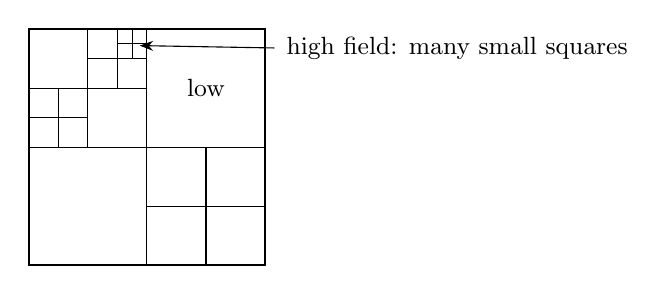
\begin{tikzpicture}[scale=3.0]
  \draw[line width=0.8pt] (0,0) rectangle (1,1);
  \draw (0.5,0)--(0.5,1); \draw (0,0.5)--(1,0.5);
  % refine the upper-left quarter
  \draw (0.25,0.5)--(0.25,1); \draw (0,0.75)--(0.5,0.75);
  % refine one of its children twice
  \draw (0.375,0.75)--(0.375,1); \draw (0.25,0.875)--(0.5,0.875);
  \draw (0.4375,0.875)--(0.4375,1); \draw (0.375,0.9375)--(0.5,0.9375);
  % refine another child once
  \draw (0.125,0.5)--(0.125,0.75); \draw (0,0.625)--(0.25,0.625);
  % refine the lower-right quarter once
  \draw (0.75,0)--(0.75,0.5); \draw (0.5,0.25)--(1,0.25);
  \node[font=\small] at (0.75,0.75) {low};
  \node[font=\small,anchor=west] at (1.05,0.92) {high field: many small squares};
  \draw[->,>=Stealth] (1.04,0.92)--(0.47,0.93);
\end{tikzpicture}
\caption{A schematic dyadic subdivision. A square is cut while $e^{h_S/Q}|S|>\varepsilon$, so the
subdivision is finest where the field is high. Here $N=19$.}
\label{fig:subdivision}
\end{figure}

Intuitively, $e^{h_S/Q}|S|$ is the size of $S$ as seen by the field: where $h$ is high, squares
count as large and are cut again and again. The final squares play the role of the faces of a
random planar map (Section~\ref{sec:intro}), and $N$ is the size of the surface. The parameter $Q$ enters only through the
rule~\eqref{eq:rule}. Duplantier and Sheffield used the same subdivisions in their proof of a
version of the KPZ relation~\cite{DS}. The \emph{height} of $S$,
\begin{equation}\label{eq:height}
H(S)\;=\;h_S-Q\log\frac{\varepsilon}{|S|},
\end{equation}
measures how far $S$ is above the threshold: $S$ is active exactly when $H(S)>0$, and at depth $j$,
$H(S)=h_S-Qj\log2-Q\log\varepsilon$. From a square to a child the height changes by $-Q\log2$ plus
a random amount of variance about $\log2$. So the squares form a \emph{branching random walk}, a
population in which each individual (a square) has four children whose positions (heights) are
its own plus a random step. Here the steps have negative drift, the population is stopped where
the height becomes negative, and the branches are correlated because nearby squares see nearly the
same field. Section~\ref{sec:brw} studies the version without correlations.

\subsection{The parameters}

APPS tie $Q$ to the central charge $c$ by $Q^2=(25-c)/6$, so $Q\ge2$ corresponds to $c\le1$. The
probability literature writes $Q$ through a second number $\gamma\in(0,2]$, the parameter of
Liouville quantum gravity (Section~\ref{sec:upper}):
\begin{equation}\label{eq:Q}
Q^2=\frac{25-c}{6},\qquad Q=\frac2\gamma+\frac\gamma2,\qquad \gamma=Q-\sqrt{Q^2-4}.
\end{equation}
So $\gamma=2$ at $Q=2$. Squaring the second relation gives
$Q^2-2=4/\gamma^2+\gamma^2/4$. With $x=4/\gamma^2$ this reads
\begin{equation}\label{eq:xQ}
x+\frac1x\;=\;Q^2-2\;=\;\frac{13-c}{6},
\end{equation}
the KPZ relation~\eqref{eq:kpz}, with $x\ge1$ because $\gamma\le2$. So the KPZ formula says that
the tail exponent of the size equals $4/\gamma^2$. The recurring values are: for a bare surface,
$c=0$, $Q^2=25/6$, $\gamma^2=8/3$, $x=3/2$; for one spanning tree, $c=-2$, $Q^2=9/2$, $\gamma^2=2$,
$x=2$; for two curves as in a meander, $c=-4$, $Q^2=29/6$, $\gamma^2=(17-\sqrt{145})/3\approx1.6528$,
$x=\xstar$; and at the critical endpoint, $c=1$, $Q=\gamma=2$, $x=1$.


%%%%%%%%%%%%%%%%%%%%%%%%%%%%%%%%%%%%%%%%%%%%%%%%%%%%%%%%%%%%%%%%%%%%%%%%
\section{Determinant weights as a change of parameter}\label{sec:tilt}
%%%%%%%%%%%%%%%%%%%%%%%%%%%%%%%%%%%%%%%%%%%%%%%%%%%%%%%%%%%%%%%%%%%%%%%%

\subsection{Spanning trees and determinants}

By Kirchhoff's matrix-tree theorem, the number of spanning trees of a connected graph is the
product of the nonzero eigenvalues of its Laplacian matrix, divided by the number of vertices. Weighting
planar maps by the $k$-th power of this number models a surface decorated by $k$ independent
spanning trees, with central charge $c=-2k$~\cite{PaperA}.

The continuum analog replaces the graph by a surface. A smooth surface with Riemannian metric $g$
has a Laplace operator $\Delta_g$ with eigenvalues
$0=\Lambda_0<\Lambda_1\le\Lambda_2\le\cdots\to\infty$. Their product diverges but can be
renormalized: the \emph{zeta-regularized determinant} is $\det{}'_\zeta\Delta_g=e^{-\mathcal Z'(0)}$,
where $\mathcal Z(s)=\sum_{i\ge1}\Lambda_i^{-s}$ is continued analytically to $s=0$. For a metric $g=e^{2\varphi}g_0$ obtained from a smooth
reference metric $g_0$ by a smooth change of scale $\varphi$, the \emph{Polyakov--Alvarez formula}
expresses the change of the determinant:
\begin{equation}\label{eq:PA}
\log\ldet=\log\det{}'_\zeta\Delta_{g_0}-\frac1{12\pi}\int|\nabla\varphi|^2\,dA_0
-\frac1{6\pi}\int K_0\,\varphi\,dA_0+\log\operatorname{Vol}_g-\log\operatorname{Vol}_{g_0},
\end{equation}
where $K_0$ is the curvature and $dA_0$ the area element of $g_0$, and $\operatorname{Vol}$ is the
total area. The formula contains the Dirichlet energy $\int|\nabla\varphi|^2$, the same quadratic
form that appears in the density of the Gaussian free field.

\subsection{The metric of the model}

Given the final partition $\Pt$ of the subdivision, with $n$ squares, APPS replace the field by a
regularized version $h^{\Pt}$: the conditional expectation of $h$ given its $n$ averages $h_S$,
$S\in\Pt$~\cite[Definition~6.4]{APPS}. It is a finite combination
\begin{equation}\label{eq:coords}
h^{\Pt}=\sum_{S\in\Pt}a_Sf_S ,
\end{equation}
where the $f_S$ are orthonormal for $(\cdot,\cdot)_\nabla$ and, for each fixed $\Pt$, the $n$
coordinates $a_S$ are independent standard normal variables~\cite[Lemma~6.5]{APPS}. The metric of
the model is
\[
g=e^{2(h^{\Pt}/Q+b)}g_0,\qquad b=\tfrac14\log n-\tfrac34\log\operatorname{Vol}_{e^{2h^{\Pt}/Q}g_0},
\]
where the constant $b$, chosen by APPS~\cite[Definition~6.7]{APPS}, rescales the total area. This
metric is not smooth, and APPS
\emph{define} its determinant $\ldet$ by the right side of~\eqref{eq:PA} with
$\varphi=h^{\Pt}/Q+b$; no spectral zeta function of the rough metric is involved.

% Source note: APPS Definition 6.4 calls h^P the finite conditional projection.

\subsection{The theorem of Ang, Park, Pfeffer and Sheffield}

\begin{theorem}[Ang, Park, Pfeffer and Sheffield {\cite[Theorem~6.9]{APPS}}]\label{thm:apps69}
Fix $n$ and a real $k$, and write $Q_k^2=Q^2+k/3$, assumed positive. Conditional on $N=n$, the law of the
subdivision at parameter $Q$, reweighted by $(\ldet)^k$, is the law of the subdivision at
parameter $Q_k$, conditioned on $N=n$.
\end{theorem}

In terms of the central charge, $Q^2\mapsto Q^2+k/3$ is $c\mapsto c-2k$: in this model, drawing $k$
spanning trees is exactly lowering the central charge by $2k$. The additivity of central charges,
an assumption for meanders, is here a theorem. The reason is visible in~\eqref{eq:PA}: the energy
term is a quadratic form in the Gaussian coordinates $a_S$, so a power of the determinant
multiplies the Gaussian density by another Gaussian factor, and only the variance changes.

\subsection{The normalization across sizes}

Theorem~\ref{thm:apps69} compares surfaces of one size. An exponent compares different sizes, so
every factor depending on $n$ matters.

\begin{proposition}[the determinant]\label{prop:det}
On the event $N=n$, with $\xi_S=a_S/Q$,
\[
\ldet\;=\;A_0\,n^{1/3}\exp\Bigl(-\frac16\sum_{S\in\Pt}\xi_S^2\Bigr),\qquad
A_0=\frac{\det{}'_\zeta\Delta_{g_0}}{\operatorname{Vol}_{g_0}} ,
\]
where $A_0$ is a deterministic constant that does not depend on $n$, $Q$ or the partition.
\end{proposition}

\begin{proof}
Put $\varphi=h^{\Pt}/Q+b$ in~\eqref{eq:PA}. The field is normalized so that its integral against
$K_0$ vanishes, and $\int K_0\,dA_0=4\pi$ by the Gauss--Bonnet theorem, so the curvature term is
$-\frac1{6\pi}\cdot4\pi b=-\frac23b$. The volume of $g$ is $e^{2b}$ times the volume of
$e^{2h^{\Pt}/Q}g_0$, so with the stated $b$ the terms outside the energy add up to
\[
-\tfrac23b+2b+\log\operatorname{Vol}_{e^{2h^{\Pt}/Q}g_0}+\log A_0=\tfrac13\log n+\log A_0 .
\]
For the energy, the orthonormality of the $f_S$ in~\eqref{eq:coords} gives
$\int|\nabla h^{\Pt}|^2=2\pi\sum_Sa_S^2$, hence
$\frac1{12\pi}\int|\nabla\varphi|^2=\frac1{6}\sum_S\xi_S^2$.
\end{proof}

The factor $n^{1/3}$ cancels when one conditions on $N=n$, so it plays no role in
Theorem~\ref{thm:apps69}. In the arXiv version of~\cite{APPS}, the display~(6.9) has $2h^\varepsilon/Q$
inside the gradient, where $h^\varepsilon$ denotes the regularized field; that is inconsistent by a factor of four with their equation~(6.7), their
Definition~6.7 and the proof of their Theorem~6.9. We derived Proposition~\ref{prop:det} from
equation~(6.7) and Definition~6.7 directly.

Write $p_n(Q)=\Prob_Q(N=n)$ for the law of the size at parameter $Q$.

\begin{proposition}[exact identity]\label{prop:identity}
Let $k$ be real with $Q_k^2=Q^2+k/3>0$. Then
\[
\E_Q\bigl[(\ldet)^k;\,N=n\bigr]\;=\;A_0^k\,n^{k/3}\Bigl(\frac{Q}{Q_k}\Bigr)^np_n(Q_k).
\]
Consequently, if $Q_k\ge2$, then for every $n$
\begin{equation}\label{eq:identity}
\sum_{n'\ge n}\Bigl(\frac{Q_k}{Q}\Bigr)^{n'}A_0^{-k}\,n'^{-k/3}\;
\E_Q\bigl[(\ldet)^k;\,N=n'\bigr]\;=\;\Prob_{Q_k}(N\ge n).
\end{equation}
\end{proposition}

\begin{proof}
Fix a partition $\Pt$ with $n$ squares. Every square that appears in the subdivision, including
the ancestors of the squares of $\Pt$, has an average that is a fixed linear combination of the
$n$ averages over $\Pt$, and these are linear in the coordinates $a_S$. The rule~\eqref{eq:rule}
reads $h_S/Q>\log(\varepsilon/|S|)$. So the event $\{\Pt^\varepsilon=\Pt\}$ is the event that the
vector $\xi=(\xi_S)_{S\in\Pt}$ lies in a set $\mathcal D_{\Pt}\subset\mathbb R^n$ that does not depend on
$Q$~\cite[Lemma~6.3]{APPS}. The vector $\xi$ has density $(Q/\sqrt{2\pi})^ne^{-Q^2|\xi|^2/2}$.
There are finitely many partitions with $n$ squares, so
\[
p_n(Q)=\Bigl(\frac Q{\sqrt{2\pi}}\Bigr)^n\sum_{\Pt:\,|\Pt|=n}\int_{\mathcal D_{\Pt}}e^{-Q^2|\xi|^2/2}\,d\xi .
\]
By Proposition~\ref{prop:det}, $(\ldet)^k=A_0^kn^{k/3}e^{-(k/3)|\xi|^2/2}$ on $N=n$. Multiplying
the density by this factor replaces $Q^2$ by $Q^2+k/3=Q_k^2$ in the exponent, which gives the
first formula. Multiply it by $(Q_k/Q)^nA_0^{-k}n^{-k/3}$ and sum over $n'\ge n$: the right side
becomes $\sum_{n'\ge n}p_{n'}(Q_k)$, which is $\Prob_{Q_k}(N\ge n)$ because $N$ is finite almost
surely at parameter $Q_k\ge2$. All terms are nonnegative, so no question of convergence arises.
\end{proof}

The identity~\eqref{eq:identity} needs two compensations. The factor $(Q_k/Q)^{n}$ is exponential:
like $\mu^n$ for meanders, it changes the growth rate but not the exponent, and we divide it out as
one divides $M_n$ by $\mu^n$. The polynomial factor $n^{-k/3}$ is essential. Without it the left
side of~\eqref{eq:identity} becomes $\E_{Q_k}[N^{k/3};N\ge n]$, and a tail $n^{-x+o(1)}$ turns this
into $n^{k/3-x+o(1)}$: the exponent shifts by $k/3$. The factor is invisible at a fixed size and
decisive across sizes.

%%%%%%%%%%%%%%%%%%%%%%%%%%%%%%%%%%%%%%%%%%%%%%%%%%%%%%%%%%%%%%%%%%%%%%%%
\section{The tail law}\label{sec:tail}
%%%%%%%%%%%%%%%%%%%%%%%%%%%%%%%%%%%%%%%%%%%%%%%%%%%%%%%%%%%%%%%%%%%%%%%%

\subsection{Statements}

The exact identity~\eqref{eq:identity} turns determinant weights into the tail of the size $N$ at a
shifted parameter. That tail is the following.

\begin{theorem}[tail law]\label{thm:tail}
For every $Q\ge2$ and every fixed $\varepsilon>0$,
\[
\lim_{n\to\infty}\frac{\log\Prob_Q(N\ge n)}{\log n}\;=\;-\frac4{\gamma^2},
\]
where $\gamma=Q-\sqrt{Q^2-4}$ as in~\eqref{eq:Q}; at the critical endpoint $Q=2$, $\gamma=2$ and
the limit is $-1$.
\end{theorem}

This is a logarithmic asymptotic, $\Prob(N\ge n)=n^{-4/\gamma^2+o(1)}$, not a limit of
$n^{4/\gamma^2}\Prob(N\ge n)$. At $Q=2$ we also prove $\E[N]<\infty$, so there the tail is not a
constant times $1/n$. With Proposition~\ref{prop:identity}, the theorem gives the KPZ formula in
the model.

\begin{theorem}[the KPZ curve]\label{thm:kpz}
Take the base parameter $Q_0^2=25/6$, that is $c=0$. For every real $k\ge-1/2$, put
$Q_k^2=Q_0^2+k/3$ and
\[
W_k(n)=\sum_{n'\ge n}\Bigl(\frac{Q_k}{Q_0}\Bigr)^{n'}A_0^{-k}\,n'^{-k/3}\;
\E_{Q_0}\bigl[(\ldet)^k;\,N=n'\bigr],
\]
the weight of surfaces with at least $n$ squares under the $k$-th power of the determinant, with
both compensations of Section~\ref{sec:tilt}. Then $W_k(n)=n^{-x_k+o(1)}$, where
\[
x_k+\frac1{x_k}=\frac{13+2k}{6},\qquad x_k\ge1,\qquad
x_k=\frac{13+2k+\sqrt{(13+2k)^2-144}}{12}.
\]
At $k=0,1,2$ this gives $x_k=3/2$, $2$ and $\xstar=(17+\sqrt{145})/12$, so $1+x_2=\astar$.
\end{theorem}

\begin{proof}
By~\eqref{eq:identity}, $W_k(n)=\Prob_{Q_k}(N\ge n)$; this needs $Q_k\ge2$, which is
$25/6+k/3\ge4$, that is $k\ge-1/2$. By Theorem~\ref{thm:tail} at parameter $Q_k$, the tail
exponent is $x_k=4/\gamma_k^2$ with $Q_k=2/\gamma_k+\gamma_k/2$, and by~\eqref{eq:xQ},
$x_k+1/x_k=Q_k^2-2=(13+2k)/6$.
\end{proof}

\begin{figure}[b]
\centering
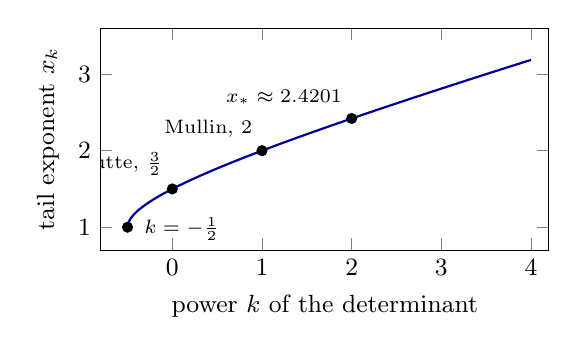
\begin{tikzpicture}
\begin{axis}[width=0.6\textwidth,height=4.4cm,xmin=-0.8,xmax=4.2,ymin=0.7,ymax=3.6,
  xlabel={power $k$ of the determinant},ylabel={tail exponent $x_k$},
  tick label style={font=\small},label style={font=\small},
  xtick={0,1,2,3,4},ytick={1,2,3}]
\addplot[domain=-0.5:4,samples=200,thick,blue!60!black]
  {(13+2*x+sqrt(max(0,(13+2*x)^2-144)))/12};
\addplot[only marks,mark=*,mark size=1.8pt] coordinates {(-0.5,1) (0,1.5) (1,2) (2,2.42013)};
\node[font=\scriptsize,anchor=west] at (axis cs:-0.42,0.98) {$k=-\frac12$};
\node[font=\scriptsize,anchor=south east] at (axis cs:0,1.55) {Tutte, $\frac32$};
\node[font=\scriptsize,anchor=south east] at (axis cs:1,2.05) {Mullin, $2$};
\node[font=\scriptsize,anchor=south east] at (axis cs:2,2.47) {$\xstar\approx2.4201$};
\end{axis}
\end{tikzpicture}
\caption{The KPZ curve of Theorem~\ref{thm:kpz}, with central charge $c=-2k$. Marked: the
critical endpoint, the bare surface, one spanning tree, and the analog of two spanning trees,
whose exponent is the meander value $\xstar=\astar-1$.}
\label{fig:kpz}
\end{figure}

Figure~\ref{fig:kpz} shows the curve. Three caveats. First, the result concerns cumulative weights,
up to factors $n^{o(1)}$; a local upper bound $\Prob(N=n)\le n^{-1-4/\gamma^2+o(1)}$ along
$n\equiv1\pmod3$ is also proved, and the local lower bound is open. So at $k=2$ it proves the
tail exponent $\xstar$, not the local exponent $\astar=1+\xstar$. Second, it is a statement for
each fixed $k$ and cannot be differentiated in $k$. Third, it concerns a continuum model in which
spanning trees are replaced by a determinant, not meanders or tree-weighted planar maps.

\subsection{A heuristic for the exponent}\label{sec:heuristic}

The proofs make the following heuristic rigorous. The size $N$ is large only if the field is
unusually high somewhere. The cheapest way is to make a single square very high and let its
descendants multiply. Two exponential rates describe this.

\emph{The cost of a high square.} Measure the growth of an average along nested squares per level,
in units of $\log2$, and call it the \emph{slope}. A square of depth $j$ whose average has slope
$\lambda$, that is $h_S\approx\lambda\,j\log2$, has height $H(S)\approx(\lambda-Q)\,j\log2$ by~\eqref{eq:height}.
There are $4^j$ squares at depth $j$, and a normal variable of variance $j\log2$ exceeds
$\lambda j\log2$ with probability about $2^{-j\lambda^2/2}$. So the expected number of squares
at height $y=(\lambda-Q)j\log2$ is about
\[
2^{\,j(2-\lambda^2/2)}=\exp\Bigl(-y\,\frac{\lambda^2/2-2}{\lambda-Q}\Bigr).
\]
Minimizing the ratio over $\lambda>Q$ gives the condition $\lambda^2/2-Q\lambda+2=0$, whose root
above $Q$ is $\lambda_+=Q+\sqrt{Q^2-4}$, and there the ratio equals $\lambda_+$. So a square of
height $y$ appears with probability about $e^{-\lambda_+y}$.

\emph{The yield of a high square.} Start from one square of height $y$ and follow its descendants
whose averages grow with slope $\theta$ below the threshold slope $Q$. Along such a path the
height decreases by $(Q-\theta)\log2$ per level, so the path stays active for about
$j'=y/((Q-\theta)\log2)$ levels. The expected number of such descendants is
\[
2^{\,j'(2-\theta^2/2)}=\exp\Bigl(y\,\frac{2-\theta^2/2}{Q-\theta}\Bigr).
\]
Maximizing over $\theta$ gives the same condition, $\theta^2/2-Q\theta+2=0$, now with the root
below $Q$, which is $\lambda_-=Q-\sqrt{Q^2-4}=\gamma$, and there the ratio equals $\gamma$. So a
square of height $y$ produces about $e^{\gamma y}$ final squares; this count is typical, not only an
expectation, because $\gamma<2$.

Putting $n=e^{\gamma y}$, the probability of at least $n$ squares is about
$e^{-\lambda_+y}=n^{-\lambda_+/\gamma}$. Since $\lambda_+\lambda_-=4$, the exponent is
$\lambda_+/\gamma=4/\gamma^2$. In words: the two roots of one quadratic,
\begin{equation}\label{eq:quadratic}
\psi(\theta)=2-Q\theta+\frac{\theta^2}2,\qquad \psi(\gamma)=\psi(4/\gamma)=0,
\end{equation}
are the rate at which height is gained cheaply and the rate at which it is spent productively,
and their ratio is the KPZ exponent. The function $\psi$ also governs the upper bound: the number
of active squares at depth $j$ is at most $2^{j\psi(\theta)}$ times a random factor with controlled
moments, for each $\theta$, as the next section shows.

The proof has four parts: the upper bound for $Q>2$, by moments of Gaussian multiplicative chaos
(Section~\ref{sec:upper}, nearly in full); the upper bound at $Q=2$, by a Brownian estimate
(Section~\ref{sec:upper}); and the lower bounds for $Q>2$ and $Q=2$, by a second-moment count of
high squares with many descendants (sketched in Section~\ref{sec:lower}).

%%%%%%%%%%%%%%%%%%%%%%%%%%%%%%%%%%%%%%%%%%%%%%%%%%%%%%%%%%%%%%%%%%%%%%%%
\section{Proof of the upper bound}\label{sec:upper}
%%%%%%%%%%%%%%%%%%%%%%%%%%%%%%%%%%%%%%%%%%%%%%%%%%%%%%%%%%%%%%%%%%%%%%%%

\subsection{Gaussian multiplicative chaos}

Let $\Phi$ be a centered Gaussian field on a square whose covariance is $-\log|z-w|$ plus a bounded
function, such as the Gaussian free field. For $0<\theta<2$, the random measure
\[
e^{\theta \Phi(z)-\theta^2\E[\Phi(z)^2]/2}\,dz ,
\]
defined by smoothing $\Phi$ at scale $r$ and letting $r\to0$, is a nonzero random measure called
\emph{Gaussian multiplicative chaos}~\cite{RV}; subtracting half the variance makes the expected
density one. Its total mass over a fixed square has a heavy tail: the moment of order $p>0$ is
finite exactly when $p<4/\theta^2$~\cite[Theorem~2.11]{RV}. Intuitively, the mass can be carried by
a small region where $\Phi$ is unusually high. For $\Phi=h$ and $\theta=\gamma$ this measure is the
\emph{Liouville quantum gravity area}. \emph{Liouville quantum gravity} (LQG) with parameter $\gamma$
is the name for a random surface whose area element is, formally, $e^{\gamma h(z)}dz$; the chaos
construction makes this precise. It is used in Sections~\ref{sec:area} and~\ref{sec:limit}.

Two further facts are used. \emph{Kahane's convexity inequality}: if two centered Gaussian fields
$\Phi$ and $\Psi$ satisfy $\operatorname{Cov}(\Phi(z),\Phi(w))\le\operatorname{Cov}(\Psi(z),\Psi(w))$
for all $z,w$, then $\E[F(m_\Phi)]\le\E[F(m_\Psi)]$ for every convex
function $F$ of at most polynomial growth, where $m_\Phi$ and $m_\Psi$ are the total masses of the two
chaos measures with the same $\theta$~\cite[Theorem~2.1]{RV}. Intuitively, more correlation makes
the mass more variable. And for a field built from independent contributions of successive scales,
the masses at finer cutoffs form a martingale, uniformly integrable when
$\theta<2$~\cite[Theorem~2.5]{RV}.

\subsection{Uniform moments of the square counts}

For $\theta>0$ and a depth $j$, define the normalized sum over the $4^j$ squares of depth $j$,
\[
\mathcal M_{\theta,j}=4^{-j}\sum_{|S|=2^{-j}}\exp\Bigl(\theta h_S-\frac{\theta^2}2\operatorname{Var}(h_S)\Bigr).
\]
It is the total mass of the chaos measure of the piecewise constant field $\Phi_j(z)=h_{S_j(z)}$,
where $S_j(z)$ is the depth-$j$ square containing $z$.

\begin{lemma}\label{lem:moments}
If $0<\theta<2$ and $1\le p<4/\theta^2$, then $\sup_j\E[\mathcal M_{\theta,j}^p]<\infty$.
\end{lemma}

\begin{proof}[Proof sketch]
The covariance of the square averages gives, uniformly in $j$, $z$ and $w$,
\[
\operatorname{Cov}\bigl(\Phi_j(z),\Phi_j(w)\bigr)\le\log\frac1{|z-w|\vee2^{-j}}+C_0 .
\]
For comparison, take the field $\Psi_u$ with covariance $\int_0^ue^{-e^{2v}|z-w|^2/2}\,dv$, which has
independent scale increments; at $u=j\log2$ this covariance is $\log(1/(|z-w|\vee2^{-j}))+O(1)$.
Adding one independent centered normal variable of large fixed variance makes its covariance dominate that of $\Phi_j$ everywhere. Kahane's inequality with
$F(u)=u^p$ bounds $\E[\mathcal M_{\theta,j}^p]$ by the $p$-th moment of the comparison mass, times a
fixed lognormal moment. The comparison masses form a uniformly integrable martingale in $u$, so
each is the conditional expectation of the limiting chaos mass, and by Jensen's inequality its $p$-th
moment is at most that of the limit, which is finite because $p<4/\theta^2$. The passage from
Kahane's inequality for finite Gaussian vectors to these integrals is routine.
\end{proof}

\subsection{The upper bound for \texorpdfstring{$Q>2$}{Q>2}}

\begin{theorem}\label{thm:upper}
Let $Q>2$ and $x=4/\gamma^2$. Then $\E[N^p]<\infty$ for every real $1\le p<x$. Consequently
\[
\limsup_{n\to\infty}\frac{\log\Prob(N\ge n)}{\log n}\le-\frac4{\gamma^2}.
\]
\end{theorem}

\begin{proof}
Let $\mathcal N_j$ be the number of squares of depth $j$ that are active, whether or not they are reached
by the subdivision. Every square that is cut in the subdivision is active, and each cut adds
three squares, so
\[
N\le1+3\sum_{j\ge0}\mathcal N_j .
\]
For any $\theta>0$, the indicator of $\{e^{h_S/Q}2^{-j}>\varepsilon\}$ is at most
$(e^{h_S/Q}2^{-j}/\varepsilon)^{\theta Q}$, so
\[
\mathcal N_j\le\varepsilon^{-\theta Q}\,2^{-\theta Qj}\sum_{|S|=2^{-j}}e^{\theta h_S}.
\]
Since $\operatorname{Var}(h_S)=j\log2+O(1)$ uniformly, $e^{\theta h_S}\le
C\,2^{j\theta^2/2}\exp(\theta h_S-\theta^2\operatorname{Var}(h_S)/2)$, and therefore
\begin{equation}\label{eq:Ij}
\mathcal N_j\;\le\;C\,2^{\,j(2-\theta Q+\theta^2/2)}\,\mathcal M_{\theta,j}=C\,2^{\,j\psi(\theta)}\mathcal M_{\theta,j},
\end{equation}
with $\psi$ the quadratic~\eqref{eq:quadratic} and $C$ depending on $\theta$, $Q$ and $\varepsilon$.

The roots of $\psi$ are $\gamma$ and $4/\gamma$, and $\psi<0$ strictly between them. Fix $p<x$. Since
$\gamma<2$ we can choose $\theta$ slightly above $\gamma$ with $\theta<2$ and $p<4/\theta^2$; then
$\psi(\theta)<0$. By Minkowski's inequality, \eqref{eq:Ij} and Lemma~\ref{lem:moments},
\[
\|N\|_p\le1+3\sum_{j\ge0}\|\mathcal N_j\|_p\le1+C\sum_{j\ge0}2^{j\psi(\theta)}\sup_i\|\mathcal M_{\theta,i}\|_p<\infty .
\]
Markov's inequality gives $\Prob(N\ge n)\le\E[N^p]\,n^{-p}$. Letting $p$ increase to $x$ proves the
bound on the limit superior.
\end{proof}

\subsection{The upper bound at the critical endpoint}

At $Q=2$ we have $x=1$, so Minkowski's inequality is not available for the needed moments below
one. Instead:

\begin{proposition}\label{prop:critupper}
At $Q=2$ and every fixed $\varepsilon>0$, $\E[N]<\infty$. Hence $\Prob(N\ge n)\le\E[N]/n$.
\end{proposition}

\begin{proof}[Proof sketch]
Let $\mathcal R_j$ count the squares of depth $j$ that are active together with all their ancestors.
Then $N\le1+3\sum_j\mathcal R_j$, and $\E[\mathcal R_j]\le4^j\sup\Prob(\mathcal A_j)$, where $\mathcal A_j$ is the event that all squares of
a fixed chain $S_0\supset\cdots\supset S_j$ are active, that is $h_{S_l}>2l\log2+2\log\varepsilon$.

Change the law by the density $\exp(2h_{S_j}-2\operatorname{Var}(h_{S_j}))$, an exponential tilt.
This gives
\[
4^j\Prob(\mathcal A_j)\le C\,\E^*\bigl[e^{-2(h_{S_j}-2j\log2)}\,;\mathcal A_j\bigr],
\]
where $\E^*$ is the tilted expectation. Under the tilt, the field's averages over circles
centered in $S_j$ with radii $r_02^{-l}$ form a Brownian motion in the variable $l\log2$, with
drift exactly $2$, plus an independent normal starting value; the square averages differ from the
circle averages by Gaussian amounts of bounded variance. The threshold also has slope $2$. So,
relative to the threshold, the averages along the chain of ancestors form a Brownian motion
$\mathcal W$ without drift, which must stay above a barrier for a time $j\log2$. Up to the bounded
errors, $e^{-2(h_{S_j}-2j\log2)}$ is $e^{-2\mathcal W_{j\log2}}$.
Allow the errors to reach $O(\sqrt{\log j})$, at the cost of an event of probability
$O(j^{-M})$ for any fixed $M$. The reflection principle gives
\[
\E\bigl[e^{-2\mathcal W_{j\log2}};\min_{u\le j\log2}\mathcal W_u\ge-b'\bigr]\le C\,b'\,e^{2b'}\,(j\log2)^{-3/2}\qquad(b'\ge1).
\]
With $b'$ of order $\sqrt{\log j}$, this yields $\E[\mathcal R_j]\le j^{-3/2+o(1)}$, which is summable.
\end{proof}

Intuitively, at the critical point the factor $4$ in the number of squares per level exactly
balances the cost of staying active, and what remains is the probability $j^{-3/2}$ that a
driftless walk stays above a barrier and ends near it.

%%%%%%%%%%%%%%%%%%%%%%%%%%%%%%%%%%%%%%%%%%%%%%%%%%%%%%%%%%%%%%%%%%%%%%%%
\section{Sketch of the lower bound}\label{sec:lower}
%%%%%%%%%%%%%%%%%%%%%%%%%%%%%%%%%%%%%%%%%%%%%%%%%%%%%%%%%%%%%%%%%%%%%%%%

\begin{theorem}\label{thm:lower}
For every $Q\ge2$ and fixed $\varepsilon>0$,
$\liminf_{n\to\infty}\log\Prob(N\ge n)/\log n\ge-4/\gamma^2$.
\end{theorem}

With Theorem~\ref{thm:upper} and Proposition~\ref{prop:critupper} this proves
Theorem~\ref{thm:tail}. We explain the structure and the key estimates; the complete argument is in
the files listed in Appendix~\ref{app:repo}. First let $Q>2$ and write
\[
\lambda_+=Q+\sqrt{Q^2-4}=\frac4\gamma,\qquad\lambda_-=Q-\sqrt{Q^2-4}=\gamma .
\]

\subsection{The difficulty with selecting a high square}

The heuristic says: find a square of large height, then count its descendants. But a high square
counts only if it is \emph{reachable}, that is, all its ancestors are active. And if one selects
``the first high square the subdivision finds'', the selection depends on the field around it, so
its descendants no longer have the simple Gaussian law of a fixed square. The proof instead counts
\emph{deterministic} squares, fixed in advance rather than found by the field, with three properties, each with a clean conditional probability
given the square's own average, and controls the count by a second moment.

\subsection{The candidates}

Fix a depth $j$. For each of the $4^j$ squares $S$ of depth $j$ consider the \emph{high band}
\[
B_S=\bigl\{h_S\in[\lambda_+j\log2,\;\lambda_+j\log2+1]\bigr\}.
\]
On $B_S$ the height of $S$ is about $y_j=\sqrt{Q^2-4}\;j\log2-Q\log\varepsilon$. Since
$\operatorname{Var}(h_S)=j\log2+O(1)$, the expected number $Z_j$ of squares in the high band is
\[
\E[Z_j]=2^{\,j(2-\lambda_+^2/2)+O(\log j)}=e^{-(\lambda_++o(1))y_j},
\]
where the last step uses $\lambda_+^2/2-2=\lambda_+(\lambda_+-Q)$, which is the statement
$\psi(\lambda_+)=0$. This is the cost $e^{-\lambda_+y}$ of the heuristic.

\emph{Reachability.} Conditional on $B_S$, the average over the ancestor of $S$ at depth $l$ is
normal with mean $\lambda_+l\log2+O(1)$ and variance at most $l\log2+O(1)$, uniformly. The
ancestor is active when this exceeds $Ql\log2+Q\log\varepsilon$, and $\lambda_+>Q$, so failure at
level $l$ has probability decaying exponentially in $l$. A compactness argument shows that all ancestors are
active with conditional probability at least some $c_0>0$ independent of $S$ and $j$. It uses a
\emph{Cameron--Martin shift}: adding to the field a smooth deterministic function, here one that
raises every relevant average by the same amount, changes the law of the field only by an explicit
density.

\emph{The ancestral ceiling.} This property keeps the ancestors of $S$ from being much higher than
needed. Fix a small $\varpi>0$ and let $\mathcal C_S$ be the event that the average
over every ancestor at depth $l\le j$ is at most $\lambda_+l\log2+\varpi j\log2$. Given $B_S$ the
ancestors follow their conditional means closely, so $\mathcal C_S$ fails with conditional probability
$o(1)$.

\emph{Many descendants.} $S$ has at least $e^{(\gamma-o(1))y_j}$ descendants all of whose ancestors
from $S$ down are active; given $B_S$ this has conditional probability tending to one
(Lemma~\ref{lem:desc}).

\subsection{The second moment and the role of the ceiling}

Let $T_j$ count the squares with $B_S\cap \mathcal C_S$. Sum over pairs $S,S'$ of depth-$j$ squares at distance
about $2^{-j_0}$; there are about $4^{2j-j_0}$ of them. Let $U$ be the ancestor of $S$ at depth $j_0$.
The averages over $S$, $S'$ and $U$ have covariances $j_0\log2+O(1)$ with each other, so
$h_S+h_{S'}-h_U$ has variance $(2j-j_0)\log2+O(1)$. If both squares are in the high band and the
ceiling holds at $U$, then $h_S+h_{S'}-h_U\ge\lambda_+(2j-j_0)\log2-\varpi j\log2$, and a
one-dimensional Gaussian bound gives
\[
\Prob(B_S\cap \mathcal C_S\cap B_{S'})\le C\,2^{-\lambda_+^2(j-j_0/2)+\lambda_+\varpi j}.
\]
Summing over $j_0$, each separation contributes at most $2^{\lambda_+\varpi j}\E[Z_j]$ up to constants,
because $2-\lambda_+^2/2<0$. Hence
\[
\E[T_j^2]\le\mathrm{poly}(j)\;2^{\lambda_+\varpi j}\;\E[Z_j].
\]
Without the ceiling, this second-moment bound holds only when $\lambda_+^2\ge8$, that is $c\le-2$.
For $c>-2$ the untruncated second moment is inflated by pairs of high squares whose common
ancestor at an intermediate depth is unusually high; the ceiling excludes such pairs, and it costs
only a conditional probability $o(1)$.

\subsection{The descendant lemma}

\begin{lemma}[descendants of a deterministic square]\label{lem:desc}
Let $Q\ge2$, $\lambda>Q$, and $0<\theta<\min(Q,2)$. For a deterministic square $S$ of depth $j$,
condition on $h_S\in[\lambda j\log2,\lambda j\log2+1]$, and let $y=(\lambda-Q)j\log2-Q\log\varepsilon$
be the resulting height. Then, uniformly in $S$ and in the conditioned value, with conditional
probability tending to one as $j\to\infty$, $S$ has at least $e^{(R_\theta-o(1))y}$ descendants
all of whose ancestors from $S$ downward are active, where
\[
R_\theta=\frac{2-\theta^2/2}{Q-\theta}.
\]
For $Q>2$ and $\theta=\gamma$, $R_\gamma=\gamma$.
\end{lemma}

\begin{proof}[Idea of the proof]
Let $\Phi_U=h_U-\E[h_U\mid h_S]$ for descendants $U$ of $S$; after rescaling $S$ to the unit square
these form a log-correlated family with bounded errors, uniformly in $S$. At a relative depth $j'$
slightly less than $y/((Q-\theta)\log2)$, give each descendant the weight
\[
w_U=4^{-j'}\exp\bigl(\theta \Phi_U-\theta^2\operatorname{Var}(\Phi_U)/2\bigr),
\]
and let $\mathcal M$ be the total weight. Three facts finish the argument.
(i) $\mathcal M$ is not small: all its negative moments are bounded uniformly, by Kahane's inequality with
the convex function $u\mapsto u^{-p}$ and the finiteness of negative moments of subcritical chaos
on a ball~\cite[Theorem~2.12]{RV}. So $\mathcal M\ge e^{-o(y)}$ with probability tending to one.
(ii) Bad descendants carry little weight: under the weighting, averages along the path to $U$
grow at slope $\theta$ while the threshold grows at slope $Q$, so by the choice of $j'$ the height
stays positive with room to spare, and descendants with an inactive ancestor or an unusually large
final value carry weight exponentially small in $y$.
(iii) Each good descendant has weight at most $2^{-j'(2-\theta^2/2)+o(y)}$. Dividing the good weight
by this maximum gives at least $e^{(R_\theta-o(1))y}$ good descendants. For $\theta=\gamma$, the
identity $2-\gamma^2/2=\gamma(Q-\gamma)$ gives $R_\gamma=\gamma$.
\end{proof}

Because the conditional probability tends to one, the lemma attaches to the candidates without
any conditional independence: given $B_S$, the intersection of the three properties has
probability at least $c_0-o(1)$ by the union bound.

\subsection{Assembly for \texorpdfstring{$Q>2$}{Q>2}}

Let $G_j$ count the depth-$j$ squares that are in the high band, satisfy the ceiling, are
reachable and active, and have at least $e^{(\gamma-o(1))y_j}$ active descendants. Then
$\E[G_j]\ge(c_0-o(1))\E[Z_j]$ and $G_j\le T_j$, so the Paley--Zygmund inequality gives
\[
\Prob(G_j>0)\ge\frac{\E[G_j]^2}{\E[G_j^2]}\ge\frac{(c_0-o(1))^2\,\E[Z_j]^2}{\E[T_j^2]}
\ge\exp\Bigl(-\Bigl(\lambda_++\frac{\lambda_+\varpi}{\sqrt{Q^2-4}}+o(1)\Bigr)y_j\Bigr).
\]
On $\{G_j>0\}$ the subdivision has at least $e^{(\gamma-o(1))y_j}$ squares. Monotonicity in $n$
fills in the sizes between consecutive values of $j$, and letting $\varpi\to0$ gives
$\liminf\log\Prob(N\ge n)/\log n\ge-\lambda_+/\gamma=-4/\gamma^2$.

\subsection{The critical endpoint}

At $Q=2$ the root $\lambda_+=2$ equals $Q$, and $\gamma=2$ is where subcritical chaos estimates
fail. Fix instead a slope $\lambda>2$ and a chaos parameter $\theta<2$. The reachability, ceiling
and second-moment estimates use only $\lambda>\max(Q,2)$, and the descendant lemma gives
$R_\theta=(2-\theta^2/2)/(2-\theta)=(2+\theta)/2$. The same assembly yields
\[
\liminf_{n\to\infty}\frac{\log\Prob(N\ge n)}{\log n}\ge-\frac{\lambda^2/2-2}{(\lambda-2)R_\theta}
=-\frac{\lambda+2}{2+\theta}.
\]
Letting $\lambda\downarrow2$ and $\theta\uparrow2$ gives $-1$. No critical chaos measure is needed.

%%%%%%%%%%%%%%%%%%%%%%%%%%%%%%%%%%%%%%%%%%%%%%%%%%%%%%%%%%%%%%%%%%%%%%%%
\section{Area versus number of squares}\label{sec:area}
%%%%%%%%%%%%%%%%%%%%%%%%%%%%%%%%%%%%%%%%%%%%%%%%%%%%%%%%%%%%%%%%%%%%%%%%

The field also defines an area. Let $\nu$ be the Gaussian multiplicative chaos of $h$ with
parameter $\gamma$, the measure $e^{\gamma h(z)-\gamma^2\E[h(z)^2]/2}dz$ of
Section~\ref{sec:upper}; this is the Liouville quantum gravity area of the surface. A
square $S$ has area roughly
\[
\nu(S)\approx e^{\gamma h_S-\gamma^2\log(1/|S|)/2}|S|^2=e^{\gamma h_S}|S|^{2+\gamma^2/2}
=e^{\gamma h_S}|S|^{\gamma Q},
\]
using $\gamma Q=2+\gamma^2/2$. Raising the rule~\eqref{eq:rule} to the power $\gamma Q$ shows that a
square is cut exactly when this rough area exceeds $\varepsilon^{\gamma Q}$. So one might guess that
$N$ is about $\nu(S_0)/\varepsilon^{\gamma Q}$. By a theorem of Wong~\cite{Wong}, $\Prob(\nu(S_0)>t)$
is asymptotic to a constant times $t^{-4/\gamma^2}$, the exponent of Theorem~\ref{thm:tail}. Yet
the guess is false in a precise sense.

\begin{proposition}\label{prop:area}
For every $Q>2$ and fixed $\varepsilon>0$,
\[
\liminf_{t\to\infty}\Prob\bigl(N=1\;\big|\;\nu(S_0)>t\bigr)>0 .
\]
\end{proposition}

\begin{proof}
Let $Y=h_{S_0}$ be the average over the unit square; it is a nondegenerate centered normal
variable, and $N=1$ exactly when $Y\le Q\log\varepsilon$, since then $S_0$ is not active. Write
$h(z)=Y\chi(z)+h^\perp(z)$ with $\chi(z)=\operatorname{Cov}(h(z),Y)/\operatorname{Var}(Y)$; the
residual field $h^\perp$ is independent of $Y$. On a closed subsquare $U$ in the interior of $S_0$,
$\chi$ is smooth and bounded, and $h^\perp$ still has covariance $-\log|z-w|$ plus a smooth
bounded function. So Wong's theorem applies to the chaos $\nu^\perp$ of $h^\perp$ and gives
that $t^{4/\gamma^2}\Prob(\nu^\perp(U)>t)$ has a positive limit.

The two chaos measures differ on $U$ by the factor $\exp(\gamma Y\chi(z)-\gamma^2\operatorname{Var}(Y)\chi(z)^2/2)$.
Choose a compact interval $\mathcal I$ below $Q\log\varepsilon$ with $\Prob(Y\in\mathcal I)>0$. For $Y\in\mathcal I$
this factor is at least a deterministic $d_0>0$ on $U$. By independence,
\[
\Prob\bigl(\nu(S_0)>t,\ N=1\bigr)\ge\Prob(Y\in\mathcal I)\,\Prob\bigl(\nu^\perp(U)>t/d_0\bigr),
\]
which is at least a positive constant times $t^{-4/\gamma^2}$, while $\Prob(\nu(S_0)>t)$ is at most a
constant times $t^{-4/\gamma^2}$, again by Wong's theorem. Dividing proves the claim.
\end{proof}

The rule~\eqref{eq:rule} sees the field only through averages over squares it has already made. If
the average over $S_0$ is low, the subdivision stops at once, however high the field is on fine
scales inside, while the area sees all scales. Given a large area, the proposition rules out that
$N$ is comparable to the area with conditional probability tending to one; it does not rule out a
comparison that holds with positive conditional probability. This is why the proof of
Theorem~\ref{thm:tail} works with the squares directly.

%%%%%%%%%%%%%%%%%%%%%%%%%%%%%%%%%%%%%%%%%%%%%%%%%%%%%%%%%%%%%%%%%%%%%%%%
\section{A branching random walk model}\label{sec:brw}
%%%%%%%%%%%%%%%%%%%%%%%%%%%%%%%%%%%%%%%%%%%%%%%%%%%%%%%%%%%%%%%%%%%%%%%%

A simplified model shows the mechanism of Section~\ref{sec:heuristic} in its purest form. Replace
the dyadic squares by the vertices of the rooted tree in which every vertex has four children. Attach to each vertex
other than the root an independent normal variable with mean
$-Q\log2$ and variance $\log2$, and let the \emph{position} of a vertex be $y_0$ plus the sum of these
variables along the path from the root, where $y_0=Q\log(1/\varepsilon)\ge0$ is the starting
position. A vertex is \emph{alive} if it and all its ancestors have nonnegative positions. Let $V$
be the number of alive vertices; the number of terminal vertices, the children of alive vertices
that are not alive, is $3V+1$.

This is the subdivision of Section~\ref{sec:model}, with the height as the position, except that
the field increments are replaced by independent normal steps; in the real model nearby steps are
correlated. It is a \emph{branching random walk killed at zero}: individuals that fall below zero
are removed together with their descendants, and $V$ is the total number of individuals that ever
live. For one step, the logarithm of four times its exponential moment is
\[
\log4-\theta Q\log2+\frac{\theta^2}2\log2=\psi(\theta)\log2,
\]
with $\psi$ the quadratic~\eqref{eq:quadratic}. For $Q>2$ it has the two roots
$\lambda_\pm=Q\pm\sqrt{Q^2-4}$, that is $\gamma$ and $4/\gamma$.

\begin{theorem}[A\"id\'ekon, Hu and Zindy~\cite{AHZ}]\label{thm:ahz}
For $Q>2$ and the start $y_0=0$, $\Prob(V\ge n)$ is asymptotic to a positive constant times
$n^{-x}$, where $x=\lambda_+/\lambda_-$.
% UNVERIFIED: the project checked the hypotheses of AHZ Theorem 1(ii) for the start 0 only;
% the general-start form of their theorem was not rechecked for this paper.
\end{theorem}

The roots $\lambda_+$ and $\lambda_-$ are the cost and yield rates of Section~\ref{sec:heuristic}. Since $\lambda_+\lambda_-=4$ and $\lambda_++\lambda_-=2Q$,
\[
x+\frac1x=\frac{\lambda_+^2+\lambda_-^2}{\lambda_+\lambda_-}=\frac{(2Q)^2-8}{4}=Q^2-2=\frac{13-c}6 .
\]
So the KPZ quadratic relates the two exponential rates of a killed branching random walk, and
$x=4/\gamma^2$ as in Theorem~\ref{thm:tail}. Here the probability of each size is also controlled.

\begin{theorem}\label{thm:brwlocal}
Let $Q>2$ and $y_0\ge0$. For all $n\ge1$, $\Prob(V=n)$ lies between two positive constant multiples of
$n^{-1-x}$, the constants depending on $Q$ and $y_0$. At $Q^2=29/6$ the exponent is $1+x=\astar$.
\end{theorem}

The lower bound and upper bounds $n^{-1-p}$ for every $p<x$ are proved directly; the sharp upper
bound also uses Theorem~\ref{thm:ahz}. Three ideas make the proof work. First, regard $V=V(y_0)$ as a
nondecreasing step function of the start $y_0$, a \emph{staircase}. Its successive jumps are exactly
independent, each with the law of $V(0)$, because the cluster that a newly alive vertex brings
along depends only on the unused steps below it. So the values of the staircase form a renewal
sequence, and by the renewal theorem each integer is a value with probability tending to
$1/\E[V(0)]>0$: a tail estimate becomes a local one at the cost of a constant. Second, given the
alive set, the margins by which its terminal children miss being alive are independent truncated
normal variables; this controls how long the staircase stays at a value. Third, a tilt along one
path at rate $\lambda_+$ makes one vertex high. The Gaussian free field lacks the independence in
the first two ideas, one reason why the local lower bound for the APPS model is open.

%%%%%%%%%%%%%%%%%%%%%%%%%%%%%%%%%%%%%%%%%%%%%%%%%%%%%%%%%%%%%%%%%%%%%%%%
\section{The conjectured meander limit}\label{sec:limit}
%%%%%%%%%%%%%%%%%%%%%%%%%%%%%%%%%%%%%%%%%%%%%%%%%%%%%%%%%%%%%%%%%%%%%%%%

The APPS model concerns determinants, not curves. For meanders themselves, Borga, Gwynne and Sun
proposed a precise description of a large random meander seen from far away~\cite{BGS}. This
section explains it; nothing in it is new. Close the river into a loop through infinity. River and
road are then two loops on the sphere crossing $2n$ times, and their union is a planar map whose
$2n$ vertices have degree four and are each visited once by both curves. A uniform meander of order
$n$ is thus a random planar map with two curves through every vertex, and each curve orders the
vertices.

\subsection{The surface and the curves}

A \emph{Liouville quantum gravity sphere} with parameter $\gamma\in(0,2)$ is, for our purposes, a
random measure of total mass one on the sphere, of the form $e^{\gamma h}d^2z$ for a variant $h$ of the Gaussian free
field, defined as a Gaussian multiplicative chaos as in Section~\ref{sec:upper}. The variant has
logarithmic singularities at marked points and a prescribed behavior at infinity, and its law is
weighted by a power of its total mass before the mass is normalized to one~\cite{DMS},
\cite[Section~2]{BGS}. We write $\nu$ for the area. Such spheres are the expected limits of random
planar maps. For uniform planar maps ($c=0$, $\gamma^2=8/3$) this is proved in the sense of metric
spaces: the limit of the graph distance, suitably rescaled, is the \emph{Brownian map}, a random
compact metric space~\cite{LeGall,Miermont}. For meanders the parameter is the value that~\eqref{eq:Q} assigns to
$c=-4$, namely $\gamma^2=(17-\sqrt{145})/3\approx1.6528$.

\emph{Schramm--Loewner evolutions} SLE$_\kappa$ are a one-parameter family of random fractal
curves in the plane, characterized by invariance under conformal maps and a Markov property: given
an initial piece, the rest of the curve is again an SLE$_\kappa$ in the remaining domain. The
parameter $\kappa>0$ measures how much the curve wiggles. For $\kappa\ge8$ the curve passes through
every point. SLE$_8$ is the scaling limit of the curve that runs around a uniformly
random spanning tree~\cite{LSWust}. Its whole-plane version starts and ends at infinity and visits
every point of the sphere; a fixed point is visited exactly once, almost surely. Given the surface,
a curve is \emph{traced at unit area speed} if it is parametrized by $[0,1]$ so that the region
covered during $[0,t]$ has area $t$. The two curves of the limit object are chosen independently of
each other and of the field before this parametrization; afterwards they share the area clock.

\begin{conjecture}[Borga, Gwynne and Sun {\cite[Conjecture~1.4]{BGS}}]\label{conj:bgs}
Large uniformly random meanders, with the uniform measure on vertices and a suitable rescaling of
distances, converge in law to a unit-area Liouville quantum gravity sphere with
$\gamma^2=(17-\sqrt{145})/3$, decorated by two independent whole-plane space-filling SLE$_8$
curves traced at unit area speed.
\end{conjecture}

A weaker form concerns only the orders of the crossings. A \emph{permuton} is a
probability measure on the unit square $[0,1]^2$ whose two marginals are uniform. A permutation
$\omega$ of $\{1,\ldots,2n\}$ gives one: spread mass $1/(2n)$ uniformly over each small square
$[\frac{i-1}{2n},\frac{i}{2n}]\times[\frac{\omega(i)-1}{2n},\frac{\omega(i)}{2n}]$. Permutons are the
natural limits of large permutations. For a meander, number the crossings $1,\ldots,2n$ from left
to right along the river, and let $\omega(i)$ be the position of crossing $i$ along the road,
traversed counterclockwise starting from crossing $1$, so $\omega(1)=1$~\cite[Definition~1.6]{BGS}.
In the limit object both curves start and end at the marked point $\infty$, which plays the role of
crossing $1$. Another starting crossing or direction would only rotate or reflect the cyclic road
order, which the events of Section~\ref{sec:nearsplit} do not see. In the limit object, the analogous
measure is the \emph{meandric permuton}
\[
\Pi(\mathcal A\times\mathcal B)=\nu\bigl(\eta_1(\mathcal A)\cap\eta_2(\mathcal B)\bigr),\qquad \mathcal A,\mathcal B\subset[0,1],
\]
where $\eta_1$ is the river curve and $\eta_2$ the road curve: $\Pi(\mathcal A\times\mathcal B)$ is the area of the
set of points that the river visits during the times $\mathcal A$ and the road during the times $\mathcal B$. Its
marginals are uniform because each curve is traced at unit area speed.

\begin{conjecture}[Borga, Gwynne and Sun {\cite[Conjecture~1.8]{BGS}}]\label{conj:permuton}
The permuton of a uniformly random meander of order $n$ converges in law, as $n\to\infty$, to the
meandric permuton $\Pi$.
\end{conjecture}

Both conjectures are open. BGS compute properties of the candidate limit, such as the expected
frequencies of small patterns in the permutation, but neither convergence nor the exponent
follows.

\emph{Why the conjecture is hard.} In the theory of Duplantier, Miller and Sheffield (``mating
of trees''), a $\gamma$-LQG surface and an independent
space-filling SLE$_\kappa$ with $\kappa=16/\gamma^2$ together have a simple description by a pair
of correlated Brownian motions. Call such a curve \emph{matched} to the surface. For one spanning
tree, $\gamma^2=2$ and $\kappa=8$ match. Mullin's bijection encodes a map with a spanning tree by two
walks, one tracing the tree and one its dual, and these walks converge to the pair of Brownian
motions~\cite{Sheffield,DMS}. For meanders each curve alone would call for $\gamma^2=2$, while the
pair calls for $\gamma^2\approx1.653$, whose matched curve has $\kappa=4\xstar\approx9.68$. No current
method handles curves that are not matched to the surface. The
next two sections therefore prove results about the limit object itself, which is well defined,
without any claim that meanders converge to it.

%%%%%%%%%%%%%%%%%%%%%%%%%%%%%%%%%%%%%%%%%%%%%%%%%%%%%%%%%%%%%%%%%%%%%%%%
\section{Near-splits}\label{sec:nearsplit}
%%%%%%%%%%%%%%%%%%%%%%%%%%%%%%%%%%%%%%%%%%%%%%%%%%%%%%%%%%%%%%%%%%%%%%%%

\subsection{Thin necks in finite meanders}

A meander of order $2m$ has a \emph{thin neck at the middle} if the first $2m$ of its $4m$
crossings along the river occupy $2m$ consecutive positions along the road, read cyclically;
equivalently, exactly two road arches pass over or under the gap between crossings $2m$ and
$2m+1$. A vertical line through that gap then meets the road twice, and on the sphere it is a short
closed curve cutting the surface into equal halves. Call this the \emph{zero-defect event} $F_0$:
no crossing is out of place. Write $\Prob_{2m}$ for the uniform probability on meanders of order
$2m$. Call a meander of order $2m$ a \emph{junction} if it is two meanders of order $m$ glued end
to end (Section~\ref{sec:intro}); only two arches pass over its middle gap, the short arch
joining crossings $2m$ and $2m+1$ and the long arch over it, so it is a special case of $F_0$. Since gluing
is injective, $q_m=M_m^2/M_{2m}$ is the probability that a uniform meander of order $2m$ is a
junction. Let $X_m$
be the number of meanders of order $m$ with one marked \emph{exterior} arch above the river, an
arch not nested under any other arch. Then
\begin{equation}\label{eq:F0}
\Prob_{2m}(F_0)=\frac{2X_m^2}{M_{2m}},\qquad M_m\le X_m\le\tfrac12M_{m+1},\qquad
2q_m\le\Prob_{2m}(F_0)\le\tfrac12C_r^2\,q_m ,
\end{equation}
with $C_r=\sup_nM_{n+1}/M_n<\infty$. (By parity the two arches are both above or both below the
river; given the side, meanders with $F_0$ correspond to pairs of meanders with a marked exterior
arch.) Under~\eqref{eq:conj},
\[
q_m\approx\frac{(A\mu^mm^{-\alpha})^2}{A\mu^{2m}(2m)^{-\alpha}}=A\,2^\alpha m^{-\alpha},
\]
so $\alpha$ is the exponent of a thin neck cutting a meander into equal halves~\cite{PaperA}.

\subsection{The continuum event}

Let $\Pi$ be a permuton, and read its second coordinate, the road, on the circle
$\mathbb T=\mathbb R/\mathbb Z$, since the road is a loop. Let $I=[0,1/2]$ be the first half of the river and $J_s=[s,s+1/2]$
(mod $1$) a cyclic half of the road. The \emph{off-block mass}
\[
d_\Pi(s)=\Pi\bigl(I\times(\mathbb T\setminus J_s)\bigr)+\Pi\bigl(([0,1]\setminus I)\times J_s\bigr)
\]
counts crossings in the first river half but not in $J_s$, or the other way around.
Intuitively, it measures how far the crossings are from splitting into two blocks at the cut
points $1/2$ on the river and $s$, $s+\frac12$ on the road. For the meandric permuton,
\[
d_\Pi(s)=\nu\bigl(\eta_1([0,1/2])\,\triangle\,\eta_2(J_s)\bigr),
\]
the area of the symmetric difference of the regions covered by the river in its first half of time
and by the road during $J_s$. A \emph{near-split with tolerance $\delta$} means
$\inf_sd_\Pi(s)\le\delta$. For finite meanders it is convenient to ignore thin strips around the cut
points. For
$0<\delta<1/8$, let $J_s^{+\delta}$ be the closed $\delta$-neighborhood of $J_s$ and $J_s^{-\delta}$
the set of points of $J_s$ at distance at least $\delta$ from its complement, and put
\[
d^\delta_\Pi(s)=\Pi\bigl([0,\tfrac12-\delta]\times(\mathbb T\setminus J_s^{+\delta})\bigr)
+\Pi\bigl([\tfrac12+\delta,1]\times J_s^{-\delta}\bigr),\qquad
E_\delta=\Bigl\{\inf_sd^\delta_\Pi(s)\le\delta\Bigr\}.
\]
For a permuton the two versions differ by at most $6\delta$, since by the uniform marginals a strip
of width $\delta$ has mass at most $\delta$. Hence
\begin{equation}\label{eq:sandwich}
\Bigl\{\inf_sd_\Pi(s)\le\delta\Bigr\}\subset E_\delta\subset\Bigl\{\inf_sd_\Pi(s)\le7\delta\Bigr\},
\end{equation}
and bounds on the two events are interchangeable up to a constant change of $\delta$.

\subsection{The exact finite version}

For a meander of order $n$, the \emph{centered atomic plot} $\Pi_n$ has mass $1/(2n)$ at each point
$\bigl((i-\frac12)/2n,(\omega(i)-\frac12)/2n\bigr)$; it has the same limits as the permuton.

\begin{proposition}\label{prop:micro}
For a meander of order $n$ and $0<\delta<1/(4n)$, the event $E_\delta$ for $\Pi_n$ holds exactly
when the first $n$ crossings along the river occupy $n$ consecutive positions along the road, read
cyclically. In particular, for order $2m$ and $\delta<1/(8m)$ it is the zero-defect event $F_0$,
and its probability is given by~\eqref{eq:F0}.
\end{proposition}

\begin{proof}
Each atom has mass $1/(2n)>\delta$, so $d^\delta_{\Pi_n}(s)\le\delta$ forces $d^\delta_{\Pi_n}(s)=0$. No
atom lies within $\delta$ of the river midpoint. The endpoints of $J_s$ are exactly $1/2$ apart, so
they sit alike relative to the grid of road positions, which has spacing $1/(2n)$. If neither is within $\delta$ of an
atom, $J_s^{+\delta}$ and $J_s^{-\delta}$ contain the same $n$ consecutive positions, and zero
off-block mass says that these are the first-half crossings. Otherwise $J_s^{-\delta}$ contains $n-1$
consecutive positions, all of first-half crossings, and $J_s^{+\delta}$ adds one candidate at each end;
exactly one of the two candidates is a first-half crossing, which again gives $n$ consecutive
positions. Conversely, if the first-half crossings occupy $n$ consecutive positions, take $s$ at the
midpoint between grid positions just before them; both endpoints of $J_s$ are then at distance
$1/(4n)>\delta$ from all atoms, and the off-block mass is zero.
\end{proof}

Heuristically, at resolution $\delta$ a meander looks like one of order about $1/\delta$, so by the
estimate $q_m\approx A2^\alpha m^{-\alpha}$ one expects $\Prob(E_\delta)\approx\delta^{\astar}$ in the
limit.

\subsection{The bounds}

\begin{theorem}[near-splits in the conjectured limit]\label{thm:nearsplit}
Let $\Pi$ be the meandric permuton of Section~\ref{sec:limit}, with
$\gamma^2=(17-\sqrt{145})/3$. There are constants $0<c_1\le C_1$ such that for all small $\delta>0$
\[
c_1\,\delta^{\astar}\;\le\;\Prob(\Pi\in E_\delta)\;\le\;C_1\,\delta^{\xstar+5/7},
\qquad\astar=\frac{29+\sqrt{145}}{12}\approx3.4201,\quad\xstar+\frac57\approx3.1344 .
\]
\end{theorem}

This concerns the limit object only; Section~\ref{sec:bridge} discusses finite meanders. The lower
bound has the predicted exponent, and holds for every
$\gamma\in(0,\sqrt2)$, that is, for every $x=4/\gamma^2>2$, with exponent $1+x$. The exponent of the upper bound is the best we
have reached. If the limit $\lim_{\delta\to0}\log\Prob(E_\delta)/\log\delta$ exists, it lies in
$[3.1344,3.4201]$. Two side results give context.
\begin{itemize}
\item \emph{Exact splits do not occur.} Almost surely no region covered by the river in a proper
cyclic time interval equals, up to area zero, one covered by the road; so $\Prob(E_0)=0$. (The
boundary of the region an SLE$_8$ has covered by a given time consists of SLE$_2$-type curves, and
the boundaries for two independent curves share no arc.)
\item \emph{One configuration has the sharp exponent.} The field event that two fixed disks around
the marked points $0$ and $1$ of the sphere (see below) each carry area $1/2+O(\delta)$, and the rest
$O(\delta)$, has probability $\delta^{\astar+o(1)}$.
\end{itemize}

\subsection{The lower bound}

The lower bound is proved by building the event, with four ingredients.
\emph{Two blobs suffice.} Suppose the sphere splits, up to area zero, into three regions, two
\emph{blobs} $O_1$, $O_2$ and a remainder $O_3$, with $|\nu(O_1)-1/2|\le\delta_1$ and $\nu(O_3)\le\delta_2$, and suppose each curve, after
discarding the times it spends in $O_3$, visits all of one of $O_1,O_2$ before any of the other.
Then $\inf_sd_\Pi(s)\le2\delta_1+7\delta_2$, and so $E_{2\delta_1+7\delta_2}$ holds. This is deterministic:
if both curves finish one blob before starting the other, the first half of river time and a
suitable half of road time cover roughly the same blob.

\emph{Fixed clumps are visited in blocks.} Fix two points $z_1,z_2$ and small disks of radius $r$
around them. Say a curve visits the two disks \emph{in blocks} if it fills one disk completely
before entering the other. Each curve visits $z_1$ and $z_2$ once, at different times, so by
continuity, for small $r$, it visits the two disks in blocks. Both curves do so with some probability $P_{\mathrm{blk}}(r)>0$; as the curves
are independent of the field and the area parametrization changes speeds but not orders, this holds
conditionally on any field event.

\emph{A convenient normalization of the field.} The unit-area sphere comes from a field with additive
constant fixed on the unit circle and three $\gamma$-singularities, at the marked points $0$, $1$
and $\infty$: the terms $-\gamma\log|z|$, $-\gamma\log|z-1|$ and, for $|z|>1$, $-(2Q-\gamma)\log|z|$
with $Q=2/\gamma+\gamma/2$~\cite[Definition~2.2]{BGS}. Its law is weighted by the power
$(2Q-3\gamma)/\gamma=x-2$ of its total area, where $x=4/\gamma^2$, and then normalized; the range
$\gamma\in(0,\sqrt2)$ of the lower bound is exactly $x>2$, where this power is positive. A Gaussian
change of variables rewrites this law exactly with the constant fixed on a large circle, inside
which the term from $\infty$ is constant. So near $0$ and $1$ the field is a Gaussian free field
plus the two singularities and a constant, and its restrictions to small disks around $0$ and $1$
are conditionally independent given the outside.

\emph{Pinned clumps, balance and the sphere weight.} Call a disk \emph{pinned} if it is centered at
a marked point, where the field has the singularity $-\gamma\log|z-z_0|$. The area of a pinned disk
has a heavier tail than that of an ordinary disk: by Wong's analysis of such chaos
masses~\cite{Wong}, it lies in $[t,2t]$ with probability asymptotic to a constant times
$t^{-(x-1)}$, against $t^{-x}$ for an ordinary disk. (The marked points are typical points of the
area, where the field is already high.) Given the outside, the disks at $0$ and $1$ are independent,
so both reach area of order $t$, with bounded outside area, at probability of order $t^{-2(x-1)}$. A
one-dimensional Gaussian coordinate of the field in the first disk moves its area continuously; the
two areas agree within $1$ with conditional probability of order $1/t$. Then after normalization
each disk holds area $1/2+O(1/t)$ and the rest $O(1/t)$. Finally the weight $(\text{total
area})^{x-2}$ multiplies the probability by $t^{x-2}$. Altogether
\[
t^{-2(x-1)}\cdot t^{-1}\cdot t^{\,x-2}=t^{-(1+x)} ,
\]
and with $\delta$ of order $1/t$ the first two ingredients give $\Prob(E_\delta)\ge c_1\delta^{1+x}$,
which is $\delta^{\astar}$ at $x=\xstar$. The disks have a fixed radius with $P_{\mathrm{blk}}(r)>0$; no estimate
for shrinking disks is needed.

\subsection{The upper bound}

The upper bound splits the event $\inf_sd_\Pi(s)\le\delta$, equivalent by~\eqref{eq:sandwich},
by where the area sits.
\begin{itemize}
\item \emph{Concentrated area.} If one small ball holds almost all the area, or the boundary of the
region the river covers in its first half of time is very small, the probability is at most a fixed fraction of that of the whole
event. This uses re-rooting: moving the marked points to points sampled from the area. These cases
are absorbed into the others.
\item \emph{Diffuse area with a moderate total.} If the total area $t$ before normalization is at
most $\delta^{-\vartheta}$ for a fixed $\vartheta<1$, and the boundary is macroscopic, near-agreement forces the boundaries of
the two regions to come close at arbitrarily many separated places, which for independent
SLE$_2$-type curves has probability below any power of $\delta$, by multipoint SLE estimates.
\item \emph{A large total.} If $t>\delta^{-\vartheta}$, two separated cells of a fixed mesh carry fixed
fractions of it. The worst case is two cells at the marked points, costing
$t^{-2(x-1)}$, refunded by $t^{x-2}$ from the sphere weight: net $t^{-x}$, at most $\delta^{\vartheta x}$,
with $\vartheta$ as close to one as desired.
\end{itemize}
So $\Prob(E_\delta)\le C\delta^{x-o(1)}$, one power short: the missing power is the balance factor of
the lower bound. The five-sevenths corollary cited in the appendix recovers part of this power through estimates on
retained rank integrals and a sum over configurations. This gives $x+5/7$. We do not interpret that integral estimate
as a conditional probability of visit-order agreement. The prediction $1+x=\astar$ corresponds to recovering the full factor.

%%%%%%%%%%%%%%%%%%%%%%%%%%%%%%%%%%%%%%%%%%%%%%%%%%%%%%%%%%%%%%%%%%%%%%%%
\section{Two glued disks}\label{sec:disks}
%%%%%%%%%%%%%%%%%%%%%%%%%%%%%%%%%%%%%%%%%%%%%%%%%%%%%%%%%%%%%%%%%%%%%%%%

One exact calculation makes the role of necks clear. It concerns a simpler random surface than
the meandric sphere, and its identification with the near-split event is open.

A \emph{quantum disk} is a Liouville quantum gravity surface with the topology of a disk. Besides
its area $\nu$, it has a boundary length, measured by the field along the boundary in the same way:
roughly $e^{\gamma h/2}$ times arc length, defined as a chaos on the boundary. The standard quantum
disk with prescribed boundary length $\ell$ is a canonical random surface of this kind~\cite{DMS}.
Ang and Gwynne computed the law of its area~\cite[Theorem~1.2]{AG}. For boundary length $1$ the area
has the inverse gamma density $K_{\mathrm d}t^{-1-x}e^{-\beta/t}$ on $t>0$, with $x=4/\gamma^2$ and
positive constants $K_{\mathrm d}$ and $\beta$. Adding a constant to the field multiplies areas by the square of the
factor by which it multiplies boundary lengths, so for boundary length $\ell$ the area has density
\begin{equation}\label{eq:AG}
f_\ell(t)=K_{\mathrm d}\,\ell^{2x}\,t^{-1-x}\,e^{-\beta\ell^2/t}.
\end{equation}
Such a disk typically has area of order $\ell^2$, and occasionally much more, with tail exponent
$x$. Glue two independent disks with boundary length $\ell$ along their boundaries, a sphere with a
neck of length $\ell$, and condition the total area to be one. Typically one disk is tiny; a
balanced split needs both to be unusually large for their boundary.

\begin{proposition}[two glued disks]\label{prop:disks}
Let $\nu_1,\nu_2$, the areas of the two disks, be independent with density~\eqref{eq:AG}. As $\ell\to0$ and $\delta\to0$,
\[
\Prob\bigl(|\nu_1-\tfrac12|\le\delta\;\big|\;\nu_1+\nu_2=1\bigr)\;\sim\;K_{\mathrm d}\,4^{1+x}\,\delta\,\ell^{2x}.
\]
In particular, if $\ell^2=\delta$, then this probability is asymptotic to $K_{\mathrm d}4^{1+x}\delta^{1+x}$; the same
exponent holds whenever $\ell^2$ stays between two fixed multiples of $\delta$.
\end{proposition}

\begin{proof}
Given $\nu_1+\nu_2=1$, $\nu_1$ has density $f_\ell(v)f_\ell(1-v)/g_\ell$, with
$g_\ell=\int_0^1f_\ell(v)f_\ell(1-v)\,dv$. First, $g_\ell\sim2K_{\mathrm d}\ell^{2x}$. Indeed, on $[\frac14,\frac34]$ both
factors are $O(\ell^{2x})$, so that part is $O(\ell^{4x})$. On $(0,\frac14)$, the factor
$f_\ell(1-v)/(K_{\mathrm d}\ell^{2x})$ tends to $(1-v)^{-1-x}$ uniformly, while $f_\ell$ is a probability density
whose mass concentrates near $0$ as $\ell\to0$, since $\nu_1$ has the law of $\ell^2$ times a fixed
variable; so that part is asymptotic to $K_{\mathrm d}\ell^{2x}$, and the part near $1$ is the same. Second, for
$v$ in a window around $1/2$, $f_\ell(v)f_\ell(1-v)\sim K_{\mathrm d}^2\ell^{4x}[v(1-v)]^{-1-x}$, uniformly. Hence
\[
\Prob\bigl(|\nu_1-\tfrac12|\le\delta\;\big|\;\nu_1+\nu_2=1\bigr)\sim\frac{2\delta\cdot K_{\mathrm d}^2\ell^{4x}\,4^{1+x}}{2K_{\mathrm d}\ell^{2x}}
=K_{\mathrm d}\,4^{1+x}\,\delta\,\ell^{2x}.\qedhere
\]
\end{proof}

Two costs appear: $\ell^{2x}$ for two large disks instead of one, and $\delta$ for the window. A neck just short enough to be invisible
at resolution $\delta$ bounds a region of area about $\delta$, so $\ell^2\approx\delta$, and the
probability is about
\[
\delta^{1+x}=\delta^{1+4/\gamma^2},
\]
which at the meander value of $\gamma$ is $\delta^{\astar}$: the KPZ exponent as the cost of a balanced
neck. The lower bound of Theorem~\ref{thm:nearsplit} has the same two factors: pinned clumps for the
large disks, and the Gaussian balance coordinate for $\delta$.

To apply this to near-splits one would need, and does not have: that a near-split forces a neck
of boundary length of order $\sqrt\delta$; that the sphere cut along it is comparable to two
independent disks given total area one, including the law of the neck length; and that the two
SLE$_8$ curves then visit the two sides in blocks with probability $\delta^{o(1)}$. Known theorems
that glue quantum disks into a sphere (conformal welding) produce an interface that is an
SLE$_{\gamma^2}$-type curve, and they describe matched SLE$_{16/\gamma^2}$ curves, not two
independent SLE$_8$ curves. Nor do near-splits imply thin necks
deterministically: on a round sphere, two curves that each fill one hemisphere in the first half of
their time and the other in the second half have zero off-block mass, although the halves meet
along the whole equator. A neck can only come from a probabilistic property of SLE$_8$.

%%%%%%%%%%%%%%%%%%%%%%%%%%%%%%%%%%%%%%%%%%%%%%%%%%%%%%%%%%%%%%%%%%%%%%%%
\section{Transfer to finite meanders}\label{sec:bridge}
%%%%%%%%%%%%%%%%%%%%%%%%%%%%%%%%%%%%%%%%%%%%%%%%%%%%%%%%%%%%%%%%%%%%%%%%

The number $\astar$ now appears in three proved statements: the KPZ curve of the APPS model (as
$1+x_2$), the near-split lower bound, and the glued disks. None concerns finite meanders. This section compares
the missing step with percolation, where the corresponding step was carried out, and proves what the
missing pieces would give.

\subsection{The analogy with percolation}

In site percolation on the triangular lattice, each site is open independently with probability
$1/2$. The probability that the open cluster of a site, the sites it reaches through open
neighbors, reaches distance $R$ is $R^{-5/48+o(1)}$, proved in three pieces. \emph{The continuum
exponent}: Lawler, Schramm and Werner computed it for the continuum limit, built from SLE$_6$, the
curve describing boundaries of large clusters~\cite{LSW}. \emph{Convergence}: Smirnov proved
convergence to that limit~\cite{Smirnov}. \emph{Transfer of rare events}: convergence says nothing
about small probabilities, and Kesten's scaling relations, based on splitting a rare event into
nearly independent events on nested annuli, transfer the continuum probability to the
lattice~\cite{Kesten}. Together these give the lattice theorem~\cite{LSW,SW}; no single piece
suffices.

For meanders the continuum exponent is partly done: Theorem~\ref{thm:nearsplit} has the predicted
exponent on the lower side and $\xstar+5/7\approx3.1344$ on the upper side. Convergence is open:
it is Conjecture~\ref{conj:bgs}, and even the weaker Conjecture~\ref{conj:permuton} is open. The
transfer of rare events has barely started: a meander is encoded by its two systems of arches,
above and below the river, and this encoding has no independence between scales, so there is no
analog of nested annuli. What is known is combinatorial.

\subsection{Combinatorial transfer facts}

Write $L(n)=n\log\mu-\log M_n$, which is nonnegative because $\mu=\sup_nM_n^{1/n}$, and
$D(m)=\log(M_{2m}/M_m^2)=-\log q_m$. A power law $M_n\approx A\mu^nn^{-\alpha}$ means
$L(n)\approx\alpha\log n$.

\begin{lemma}\label{lem:transfer}
The following hold for all $m,n\ge1$.
\begin{enumerate}
\item[(a)] \emph{The halving identity.} $L(n)=\sum_{j\ge0}2^{-(j+1)}D(2^jn)$.
\item[(b)] \emph{Exact neck at one-cell tolerance.} For the centered atomic plot of a meander of
order $2m$ and $0<\delta<1/(8m)$, the near-split event $E_\delta$ is the zero-defect event $F_0$,
and $2q_m\le\Prob_{2m}(E_\delta)\le\frac12C_r^2q_m$.
\item[(c)] \emph{Few mismatches cost little.} There is an absolute constant $C$ such that the number
of meanders of order $m+n$ with at most $w\ge2$ road arches crossing a given river gap, with $2m$
crossings on its left, is at most $e^{Cw}M_mM_n$.
\item[(d)] \emph{Near-splits at small tolerance.} Consequently, for the centered atomic plot of a
uniform meander of order $2m$ and every $0<\delta<1/8$,
\[
q_m\le\Prob_{2m}(E_\delta)\le e^{C(m\delta+1)}q_m .
\]
\end{enumerate}
\end{lemma}

Part (a) holds because $D(m)=2L(m)-L(2m)$, so the sum telescopes, and $L(n)/n\to0$. Part (b) is
Proposition~\ref{prop:micro} with~\eqref{eq:F0}. Part (c) is a completion argument: close each half
into a meander by a few new crossings, merging the resulting loops one by one, and record the moves
in a word of length $w-1$ over four letters from which the construction can be undone. Part (d) follows from (c), since a near-split
with tolerance $\delta$ has of order $m\delta+1$ arches over the middle gap, and because an exact
junction is a near-split. So at tolerance $w/m$ with $w=o(\log m)$, a near-split costs the exact
neck probability times $m^{o(1)}$; the continuum sees much coarser tolerances.

\subsection{The conditional lower bound}

\begin{proposition}[conditional lower bound]\label{prop:condlower}
Suppose that for some $w_n\ge1$ with $w_n/\log n\to0$, the centered atomic plot $\Pi_n$ of a
uniform meander of order $n$ satisfies
\[
\Prob\bigl(\Pi_n\in E_{w_n/n}\bigr)\;\ge\;n^{-o(1)}\;\Prob\bigl(\Pi\in E_{w_n/n}\bigr)
\]
along even $n$. Then $M_n\ge\mu^nn^{-\astar-o(1)}$ for all $n$.
\end{proposition}

\begin{proof}
Let $n=2m$ and $\delta=w_n/n$. By Lemma~\ref{lem:transfer}(d), the hypothesis and the lower bound of
Theorem~\ref{thm:nearsplit},
\[
q_m\ge e^{-C(w_n+1)}\Prob(\Pi_n\in E_\delta)\ge e^{-C(w_n+1)}n^{-o(1)}c_1\Bigl(\frac{w_n}n\Bigr)^{\astar}
=n^{-\astar-o(1)},
\]
because $w_n=o(\log n)$ and $w_n\ge1$. So $D(m)\le(\astar+o(1))\log m$ as $m\to\infty$. Insert
this into the halving identity. Every argument $2^jn$ there is at least $n$, so for large $n$ the
bound applies to every term, and since $\sum_j2^{-(j+1)}\log(2^jn)=\log n+\log2$,
\[
L(n)\le(\astar+o(1))(\log n+\log2).
\]
Hence $M_n=\mu^ne^{-L(n)}\ge\mu^nn^{-\astar-o(1)}$.
\end{proof}

The hypothesis is a \emph{relative} estimate: it compares the probabilities of polynomially rare
events, at a tolerance just above one lattice cell, for finite meanders and for the limit object. It
is much stronger than Conjecture~\ref{conj:permuton}, which concerns only typical behavior. The conclusion would be the first power-law lower
bound for meanders; the best unconditional one, $M_n\ge\mu^ne^{-K\sqrt n}$, is in Paper~C~\cite{PaperC}.
% Checked: Paper C, Theorem 1, states this bound.

\subsection{The conditional upper bound}

The other direction needs much less precision. A \emph{coupling} of two random objects is a
construction of both on one probability space. For two measures $\rho,\rho'$ on $[0,1]^2$ let
$d_{\mathrm{rect}}(\rho,\rho')=\sup|\rho(\mathcal A\times\mathcal B)-\rho'(\mathcal A\times\mathcal B)|$, the supremum over rectangles
$\mathcal A\times\mathcal B$ with $\mathcal A$ an interval of river positions and $\mathcal B$ an interval of
road positions.

\begin{proposition}[conditional upper bound]\label{prop:condupper}
Suppose that for some $\sigma,\tau>0$ and every large even $n$, the centered atomic plot $\Pi_n$ of a
uniform meander of order $n$ and the meandric permuton $\Pi$ can be built on one probability space
so that
\[
\Prob\bigl(d_{\mathrm{rect}}(\Pi_n,\Pi)>n^{-\tau}\bigr)\le Cn^{-\sigma}.
\]
Then $M_n\le C_{\alpha'}\,\mu^nn^{-\alpha'}$ for every $\alpha'<\min\bigl(\sigma,(\xstar+5/7)\,\tau\bigr)$, where
$(\xstar+5/7)\tau\approx3.1344\,\tau$.
\end{proposition}

\begin{proof}
The off-block mass $d_\rho(s)$ is a sum of the masses of at most four rectangles, so
$|d_\rho(s)-d_{\rho'}(s)|\le4d_{\mathrm{rect}}(\rho,\rho')$ for every $s$. An exact junction of an order
$n=2m$ meander has $d_{\Pi_n}(s)=0$ for a suitable $s$. So on the event of a good coupling,
$\inf_sd_\Pi(s)\le4n^{-\tau}$, and by~\eqref{eq:sandwich} and Theorem~\ref{thm:nearsplit},
\[
q_m\le Cn^{-\sigma}+\Prob\bigl(\Pi\in E_{4n^{-\tau}}\bigr)\le Cn^{-\sigma}+C'n^{-(\xstar+5/7)\tau}.
\]
Hence $D(m)\ge\alpha'\log m-O(1)$ for every $\alpha'$ below the minimum, and the halving identity
gives $L(n)\ge\alpha'\log n-O(1)$ for all large $n$.
\end{proof}

Here the tolerance $n^{-\tau}$ may be much coarser than one cell, and no completion is needed. Since
$M_n\le\mu^{n+1}/(8n)$ is known~\cite{PaperC}, this improves on known bounds only when
$\min(\sigma,3.1344\,\tau)$ exceeds one.
% Checked: Paper C, Theorem 1, states this bound.

%%%%%%%%%%%%%%%%%%%%%%%%%%%%%%%%%%%%%%%%%%%%%%%%%%%%%%%%%%%%%%%%%%%%%%%%
\section{Open problems}\label{sec:open}
%%%%%%%%%%%%%%%%%%%%%%%%%%%%%%%%%%%%%%%%%%%%%%%%%%%%%%%%%%%%%%%%%%%%%%%%

\begin{enumerate}
\item \textbf{The sharp continuum exponent.} Prove $\Prob(\Pi\in E_\delta)\le\delta^{\astar-o(1)}$ for the
meandric permuton, for instance by showing that a near-split forces a neck of boundary length of
order $\sqrt\delta$, so that the glued-disk calculation of Section~\ref{sec:disks} could finish.
% UNVERIFIED: whether improving the one-pin conditional estimate alone to delta^(1-o(1)) suffices
% for the sharp exponent is not stated in the sources; omitted here.
\item \textbf{A local law in the APPS model.} Prove $\Prob(N=n)=n^{-1-4/\gamma^2+o(1)}$ along
$n\equiv1\pmod3$; the upper bound is proved.
\item \textbf{Determinant-weighted maps.} Relate planar maps weighted by powers of their number of
spanning trees to the determinant-weighted APPS model, with enough control of rare events to
transfer Theorem~\ref{thm:kpz}.
\item \textbf{Convergence.} Prove Conjecture~\ref{conj:bgs}, or even its weaker permuton form,
Conjecture~\ref{conj:permuton}.
\item \textbf{A separation lemma.} Show that near-splits of finite meanders at moderate tolerances,
much coarser than $(\log n)/n$, are only a factor $n^{o(1)}$ more likely than exact ones, a meander
analog of Kesten's estimates. It would allow coarser tolerances in
Proposition~\ref{prop:condlower}.
\item \textbf{A quantitative coupling} as in Proposition~\ref{prop:condupper}, with a polynomial rate.
\end{enumerate}


\clearpage
\appendix
%%%%%%%%%%%%%%%%%%%%%%%%%%%%%%%%%%%%%%%%%%%%%%%%%%%%%%%%%%%%%%%%%%%%%%%%
\section{Where the proofs are}\label{app:repo}
%%%%%%%%%%%%%%%%%%%%%%%%%%%%%%%%%%%%%%%%%%%%%%%%%%%%%%%%%%%%%%%%%%%%%%%%

All proofs are in the project repository~\cite{Repo}, folder \texttt{meandric/research}. Below,
\texttt{1340}--\texttt{1343}, \texttt{623} and \texttt{626} abbreviate the folders whose names begin
with these numbers, and the extension \texttt{.md} is omitted; \texttt{1340/PROOF\_MAIN\_THEOREM} has
the dependency table for the tail law and the KPZ curve. Every result listed is \emph{checked}: a
separate, independent reading of the written proof, in the listed file, found no gap (sometimes
after clarifications that were incorporated). Nothing has been reviewed outside the project.

\begin{center}
\footnotesize\setlength{\tabcolsep}{3pt}\renewcommand{\arraystretch}{0.98}
\begin{tabular}{>{\raggedright\arraybackslash}p{0.195\textwidth}>{\raggedright\arraybackslash}p{0.395\textwidth}>{\raggedright\arraybackslash}p{0.37\textwidth}}
\toprule
result & proof & independent check\\
\midrule
Props.~\ref{prop:det}, \ref{prop:identity} (normalization) & \fn{1340/PROOF_NORMALIZATION} &
\fn{1343/REFEREE_NORMALIZATION}\\
Thm.~\ref{thm:upper} (upper bound, $Q>2$) & \fn{1341/PROOF_sharp_upper} & \fn{1343/REFEREE_SHARP_UPPER}\\
Reachability, ceiling & \fn{1341/PROOF_spine_hit} &
\fn{1343/REFEREE_SPINE_GENERAL}\\
Lemma~\ref{lem:desc} (descendants) & \fn{1340/PROOF_DESCENDANTS} &
\fn{1342/REFEREE_APPS_DESCENDANTS}, \fn{1343/REFEREE_CRITICAL_LOWER}\\
Thm.~\ref{thm:lower}, $Q>2$ (assembly) & \fn{1341/PROOF_sharp_tail_all_subcritical} &
\fn{1340/REFEREE_SHARP_TAIL_ASSEMBLY}\\
Prop.~\ref{prop:critupper} ($Q=2$ upper) & \fn{1342/PROOF_APPS_CRITICAL_UPPER} &
\fn{1340/REFEREE_CRITICAL_UPPER}\\
Thm.~\ref{thm:lower}, $Q=2$; Thm.~\ref{thm:kpz}, $k=-\frac12$ & \fn{1341/PROOF_critical_lower},
\fn{1341/PROOF_critical_tail} & \fn{1343/REFEREE_CRITICAL_LOWER}, \fn{1340/REFEREE_CRITICAL_ASSEMBLY}\\
Local upper bound & \fn{1341/PROOF_local_upper} & \fn{1343/REFEREE_LOCAL_UPPER}\\
Prop.~\ref{prop:area} (area) & \fn{1341/PROOF_area_obstruction} & \fn{1340/REFEREE_AREA_OBSTRUCTION}\\
Thm.~\ref{thm:brwlocal} (branching walk) & \fn{623/PROOF_TOY} & \fn{626/FINAL}, \fn{626/REPAIRS}\\
Identity for $d_\Pi$, \eqref{eq:sandwich} & \fn{1341/PROOF_OFFBLOCK_SET_IDENTITY} &
\fn{1342/REFEREE_TWO_DISK_BALANCE}\\
Prop.~\ref{prop:micro}, \eqref{eq:F0} & \fn{1343/PROOF_MICROSCOPIC_EQUIVALENCE},
\fn{1340/PROOF_ZERO_DEFECT} & \fn{1343/REFEREE_MICROSCOPIC_EVENT}, \fn{1343/REFEREE_ZERO_DEFECT}\\
Thm.~\ref{thm:nearsplit}, lower bound & \fn{1341/PROOF_CONTINUUM_SMALL_BALL_LOWER},
\fn{1340/PROOF_SPHERE_GAUGE_CHANGE}, \fn{1342/PROOF_PINNED_GMC_LOCAL_TAIL},
\fn{1341/LEMMA_TWO_BLOB_SUFFICIENCY}, \fn{1341/LEMMA_FIXED_CLUMP_SLE} &
\fn{1342/REFEREE_SPHERE_PINNED_CLUMPS}, \fn{1343/REFEREE_PINNED_GMC_LOCAL_TAIL},
\fn{1342/REFEREE_FIXED_CLUMP_SLE}\\
Thm.~\ref{thm:nearsplit}, upper bound & \fn{1340/PROOF_GLOBAL_NEARBLOCK_UPPER_A} (exponent
$\xstar-o(1)$), \fn{1340/COROLLARY_GLOBAL_FIVE_SEVENTHS_GAIN} ($\xstar+5/7$); intermediate steps in
\fn{1340/FINAL} & reviews named in the first file's header; \fn{1343/REFEREE_GLOBAL_FIVE_SEVENTHS_GAIN}\\
$\Prob(E_0)=0$ & \fn{1341/PROOF_EXACT_BLOCK_ZERO_BOUNDARY_TREE} &
\fn{1342/REFEREE_EXACT_BLOCK_ZERO_SKELETON}\\
Fixed two-clump event & \fn{1341/PROOF_FIXED_TWO_CLUMP_UPPER} & \fn{1342/REFEREE_FIXED_TWO_CLUMP_UPPER}\\
Prop.~\ref{prop:disks} (glued disks) & \fn{1341/PROOF_TWO_DISK_BALANCE} & \fn{1342/REFEREE_TWO_DISK_BALANCE}\\
Lemma~\ref{lem:transfer}(c), (d) & \fn{1343/PROOF_LINEAR_RECORD_COMPLETION} &
\fn{1342/REFEREE_LINEAR_RECORD_COMPLETION}\\
Prop.~\ref{prop:condlower} & \fn{1340/PROOF_ONE_SIDED_TRANSFER}, \fn{1343/PROOF_BRIDGE} &
\fn{1343/REFEREE_ONE_SIDED_TRANSFER}\\
Prop.~\ref{prop:condupper} & \fn{1342/REDUCTION_MESOSCOPIC_UPPER_TRANSPORT} &
\fn{1340/REFEREE_FINITE_RUN_AND_TRANSPORT}\\
Bounds on $M_n$ in Sec.~\ref{sec:bridge} & \fn{1340/PROOF_SQRT_COUNT_BOUND} (lower),
\fn{403_alpha_bounds/PROOF} (upper) & \fn{1341/REFEREE_SQRT_COUNT_BOUND},
\fn{404_referee_alpha_bounds/REPORT}\\
\bottomrule
\end{tabular}
\end{center}


\bibliographystyle{plain}
{\footnotesize\bibliography{../common/refs}}

\end{document}
